%
% 98-127
% Lecture 03: Wrangling Unity
% 
% Template adapted from
% https://www.cs.cmu.edu/~15150/previous-semesters/2012-spring/resources/latex/template.tex
%

\documentclass[11pt]{article}

\usepackage{amsmath}
\usepackage{amssymb}
\usepackage{amsthm}
\usepackage{hyperref}
\usepackage{fancyhdr}
\usepackage{listings}
\usepackage{color}
\usepackage{graphicx}
\usepackage{setspace}
\usepackage{times}
\usepackage{wrapfig}
\usepackage{fontawesome}

\usepackage{menukeys}

\oddsidemargin0cm
\topmargin-2cm
\textwidth16.5cm
\textheight23.5cm

\newtheorem{lemma}{Lemma}

%% Begin Constants %% <-- (edit these!)

% Lecture Info
\newcommand{\lecturenum}{3}
\newcommand{\lecturename}{Wrangling Unity}

% Author of THIS document
\newcommand{\authorname}{Adrian Biagioli}

% Course Info
\newcommand{\coursenum}{98-127}
\newcommand{\coursename}{Game Creation for People Who Want to Make Games}
\newcommand{\coursesem}{F19}

% Instructors of course
\newcommand{\instructors}{Adrian Biagioli (\,\href{mailto:abiagiol@andrew.cmu.edu}{abiagiol@andrew.cmu.edu}\,) \\ Carter Williams (\,\href{mailto:ncwillia@andrew.cmu.edu}{ncwillia@andrew.cmu.edu}\,)}

% Math shortcuts
\newcommand{\work}{\mathcal{W}}
\newcommand{\expv}{\mathbf{E}}
\newcommand{\pr}{\mathbf{Pr}}
\newcommand{\ts}{\textsuperscript}
\newcommand{\bigo}{\mathit{O}}

% Overlay image
\def\Put(#1,#2)#3{\leavevmode\makebox(0,0){\put(#1,#2){#3}}}
% Example:
% \Put(10,0){\includegraphics[width=5cm]{image-src}}

%% End Constants %%

%% Begin syntax highlighting settings %%

\definecolor{dkgreen}{rgb}{0,0.6,0}
\definecolor{gray}{rgb}{0.5,0.5,0.5}
\definecolor{mauve}{rgb}{0.58,0,0.82}

\lstset{frame=tb,
    language={[Sharp]C},
    aboveskip=3mm,
    belowskip=3mm,
    showstringspaces=false,
    columns=flexible,
    basicstyle={\small\ttfamily},
    numbers=left,
    stepnumber=1,
    numberstyle=\tiny\color{gray},
    keywordstyle=\color{blue},
    commentstyle=\color{dkgreen},
    stringstyle=\color{mauve},
    breaklines=true,
    breakatwhitespace=true,
    tabsize=3
  }

\lstnewenvironment{csharp}[1][]
{
  \lstset{frame=tb,
    language={[Sharp]C},
    aboveskip=3mm,
    belowskip=3mm,
    showstringspaces=false,
    columns=flexible,
    basicstyle={\small\ttfamily},
    numbers=left,
    stepnumber=1,
    numberstyle=\tiny\color{gray},
    keywordstyle=\color{blue},
    commentstyle=\color{dkgreen},
    stringstyle=\color{mauve},
    breaklines=true,
    breakatwhitespace=true,
    tabsize=3
  }
}{}

\lstnewenvironment{pseudocode}[1][]
{
    \lstset{
        mathescape=true,
        frame=tb,
        numbers=left, 
        basicstyle=\small, 
        numberstyle=\tiny\color{gray},
        keywordstyle=\color{black}\bfseries\em,
        commentstyle=\color{dkgreen},
        stringstyle=\color{mauve},
        keywords={,input, output, return, datatype, function, in, if, else, foreach, while, begin, end, }
        numbers=left,
        breaklines=true,
        breakatwhitespace=true,
        tabsize=3
    }
}
{}

% From https://tex.stackexchange.com/questions/95036/continue-line-numbers-in-listings-package
\def\ContinueLineNumber{\lstset{firstnumber=last}}
\def\StartLineAt#1{\lstset{firstnumber=#1}}
\let\numberLineAt\StartLineAt

%% End syntax highlighting settings %%

\setlength{\parindent}{2em}
\setlength{\parskip}{5pt plus 1pt}
\renewcommand{\baselinestretch}{1.15}

\pagestyle{fancyplain}
{
    \lhead{\fancyplain{}{Lecture \lecturenum}}
    \rhead{\fancyplain{}{\coursenum}}
    \chead{\fancyplain{}{\lecturename}}
}
\setlength{\headheight}{14pt}

\graphicspath{ {./images/} }

\begin{document}

\thispagestyle{plain}
{
    \vspace{1.5em}
    \begin{center}
    {
        \huge
        Lecture \lecturenum \\
        \vspace{0.5em}
        \lecturename
        \vspace{0.4em}
    } \\
    {
        \it
        \coursenum: \coursename\ \ (\coursesem)
    } \\
    \vspace{1.0em}
    Written by \authorname \\
    \vspace{0.7em}
    Instructors:\\ \instructors
    \end{center}
}

\section{Objectives}

By the end of this lesson you will be able to:
\begin{itemize}
    \item Create C\# scripts in the Unity editor, edit them, and apply them to GameObjects as Components
    \item Understand the basics of Unity's \lstinline|MonoBehaviour|: \lstinline|Start()|, 
          \lstinline|Update()|, and more
    \item Add easy-to-use interfaces to your component in the Unity Inspector, enabling artists and
          level designers to tweak parameters in your Unity code.
    \item Allow your scripts to inter-operate with other Components (of your own creation or 
          Unity's)
    \item Use Prefabs to dynamically create GameObjects in your scripts
\end{itemize}

\noindent These lecture notes were written for {\bf Unity 2018.3.3f1}.

\section{Downloading the Base Code}

You can download all of the base code for this lecture via the following Unitypackage.  In these 
lecture notes, I've included the path to each script before every code sample (for example, the 
first code sample below is labeled \directory{BasicFunctions/StartTester.cs}, which means that you 
can find \lstinline|StartTester.cs| in the \lstinline|BasicFunctions| folder).

\begin{center}
\href{http://stage.gamecreation.org/StuCo/F19/packages/lec03resources.unitypackage}{http://stage.gamecreation.org/StuCo/F19/packages/lec03resources.unitypackage}
\end{center}

\noindent See the lecture 2 notes for more info on how to import Unitypackages.

\pagebreak

\section{Cooking Components}

In the last lecture, we went over how to use components created by your team members or Unity 
themselves to compose complex relationships between GameObjects.  But what if we want to define our 
own custom behavior?  Unity allows you to create your own components via a \textbf{C\# Script}.  C\# 
is a programming language maintained by Microsoft.  It is very similar to Java and should feel 
familiar to anyone who knows a C-based language.  We will not cover how to code in this class; if 
you are interested in learning more about using C\#, you can find plenty of resources online.
We will try to write about important differences between C\# and C/C++/Java/Python (languages that
are used more often in classes at CMU), so do not fret if you have no experience with C\# in particular.
Read more about C\# \href{https://docs.microsoft.com/en-us/dotnet/csharp/}{here}.

To create a new component type, you need to create a C\# Script in the project view.  Open up the 
project view in Unity, right click on it, and select \menu{Create > C\# Script}.  Alternatively you 
can navigate to \menu{Assets > Create > C\# Script}.  Name your first script
\lstinline|StartTester.cs|.  Let's make this script print the familiar ``Hello, World'' to the 
debugging console.  Type the following in your editor:

\directory{BasicFunctions/StartTester.cs}
\StartLineAt{1}
\begin{csharp}
using UnityEngine;

public class StartTester : MonoBehaviour
{
    // Start() is called exactly once when you launch the game
    private void Start()
    {
        // Use Debug.Log(...) to log to the Console view
        Debug.Log("Hello, World!");
    }
}
\end{csharp}

This should look fairly familiar to those who have experience with Java or C\#.  On line 1 we see the
\lstinline|using UnityEngine| directive; this instructs C\# to bring the \lstinline|UnityEngine|
classes in scope, so that we can use them\footnote{You can think of the
\lstinline|using| keyword as similar to \lstinline|import| in Java or \lstinline|#include| in C/C++}.
Our class, called \lstinline|StartTester|, represents the component that we want to create.  You are
\textbf{required} to name the class the same as the file.  For example, because this component class
is named \lstinline|StartTester| we have to save it in \directory{StartTester.cs}.  The class derives
from the \lstinline|MonoBehaviour| base class\footnote{The colon (\lstinline|:|) operator works 
similarly to C++: it indicates in this case that \lstinline|StartTester| \textit{is a} 
\lstinline|MonoBehaviour|.  ``\lstinline|:|'' can be compared to \lstinline|extends| in Java.  More
info on this can be found in the 
\href{https://docs.microsoft.com/en-us/dotnet/csharp/programming-guide/classes-and-structs/polymorphism}{C\# documentation}.}.
\textbf{MonoBehaviour is the base class for all components}, and all components must derive from
\lstinline|MonoBehaviour| in this way\footnote{The name \lstinline|MonoBehaviour| comes from Mono,
a cross-platform community implementation of the C\# standard library and compiler (known together as 
Microsoft .NET).  Unity uses a modified version of Mono for it's compiler.}.

We have only added one function to this class, \lstinline|void Start()|.  The name \lstinline|Start|
is special for MonoBehaviours: \lstinline|Start()| is called exactly once when this component has
finished initialization.  Inside of \lstinline|Start()|, we call \lstinline|Debug.Log(string)|,
which is a Unity-provided equivalent of \lstinline|Console.Log| or \lstinline|printf|.

Now let's add our newly-created component to a GameObject.  Create an empty GameObject 
(\menu{GameObject>Create Empty}) and select it in the Hierarchy view.  Click on the \menu{Add Component}
button in the inspector, and search for ``Start Tester.''  Alternatively you can drag and drop the
\directory{StartTester.cs} file into the inspector.  Notice how Unity picked up the \lstinline|CamelCasing|
in the class name StartTester and expanded it to the more readable ``Start Tester'' name.
\begin{center}
\raisebox{-.35\height}{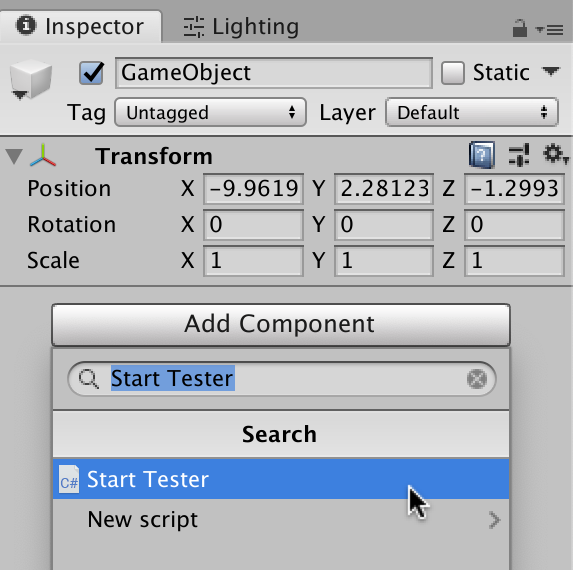
\includegraphics[width=0.35\textwidth]{add-component-1}} $\rightarrow$
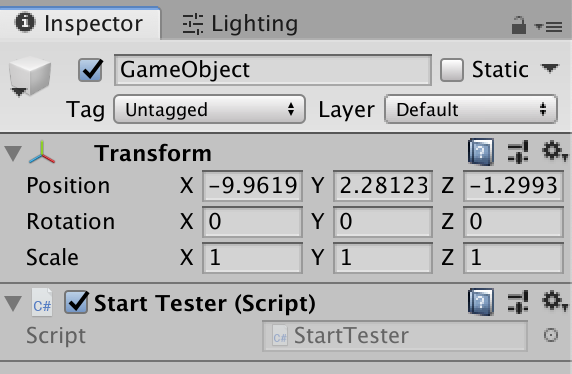
\includegraphics[width=0.35\textwidth]{add-component-2}
\end{center}

Hit the play button and you will see ``Hello, World!'' appear in the console previewer on the bottom
left of the window.  You can click on that message or navigate to \menu{Window>General>Console} to
open the Unity Console Window.  The Console keeps track of all of the \lstinline|Debug.Log| messages
that you print in your scripts as well as generally useful debugging messages from Unity components.
\begin{center}
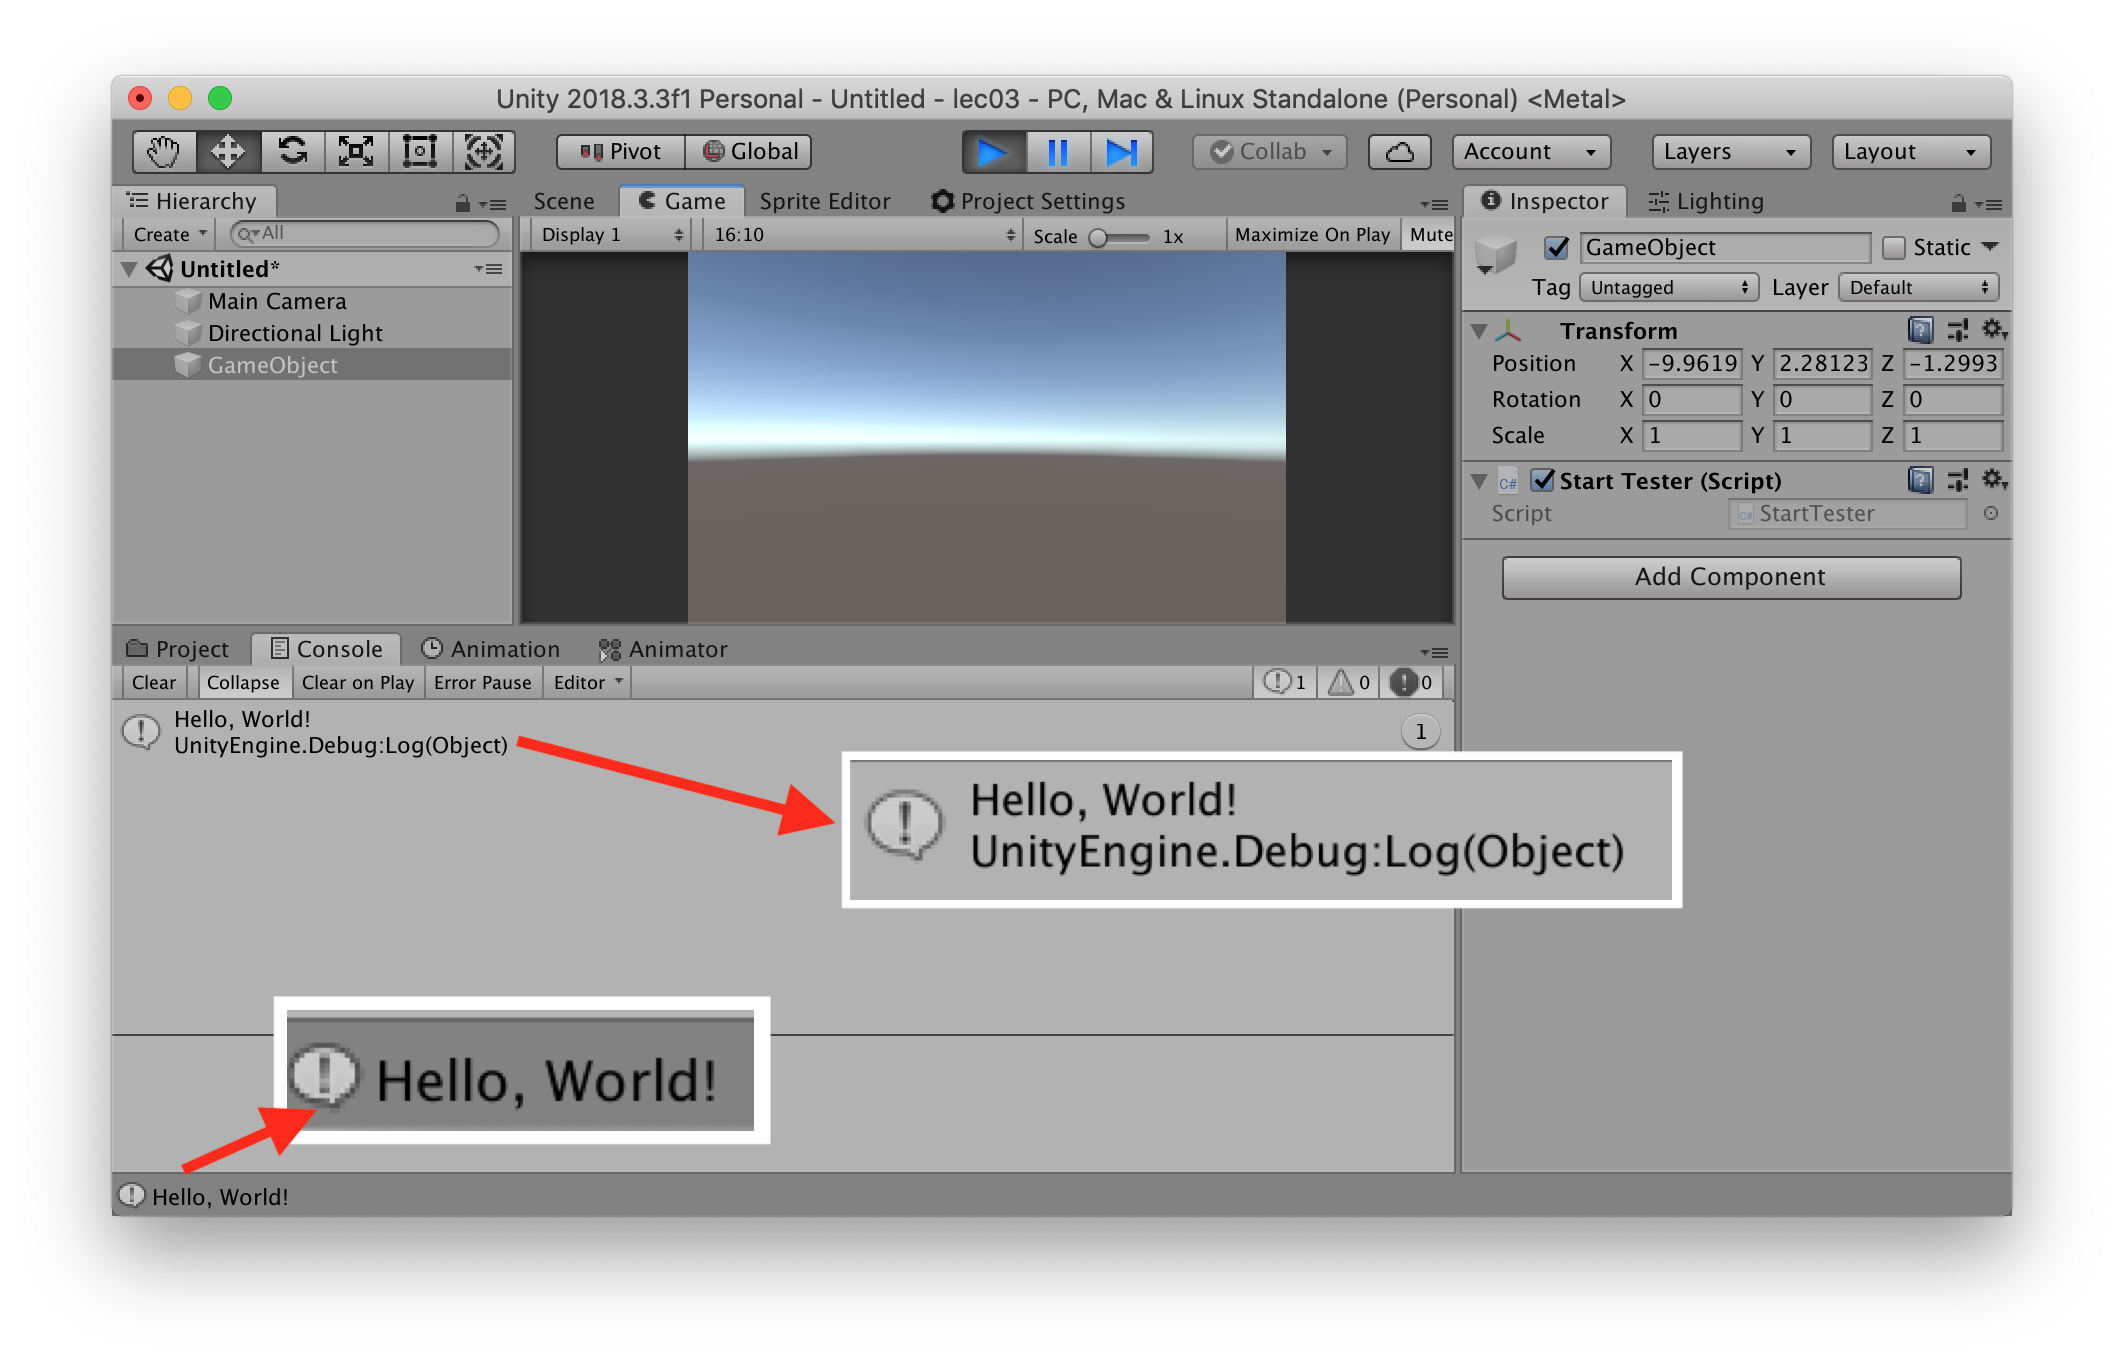
\includegraphics[width=0.8\textwidth]{start-tester} 
\end{center}

Our next example, the \lstinline|UpdateTester|, replaces \lstinline|Start| with a new function, called
\lstinline|Update()|.  \lstinline|Update| is called once per frame, unlike \lstinline|Start| which
is only called once.  Most of your game logic goes inside of \lstinline|Update|, and it is the most
straightforward way to interact with the scene over time.\pagebreak

\directory{BasicFunctions/UpdateTester.cs}
\StartLineAt{1}
\begin{csharp}
using UnityEngine;

public class UpdateTester : MonoBehaviour
{
    // Update() is called once per frame
    void Update()
    {
        Debug.Log("Hello, World! (a lot)");
    }
}
\end{csharp}

Attach this script to the empty GameObject, and watch the console get spammed by ``Hello, World!''s.
This occurs because \lstinline|Debug.Log| is being called once per frame, and there are around 60
frames per second.  Therefore we get hundreds of messages in the Console window.
You can click the \menu{Collapse} button at the top of the Console to coalesce debug messages that
come from the same line of code.  This is incredibly helpful to parse the log when multiple
\lstinline|Debug.Log|s are being called per frame!
\begin{center}
\raisebox{-.45\height}{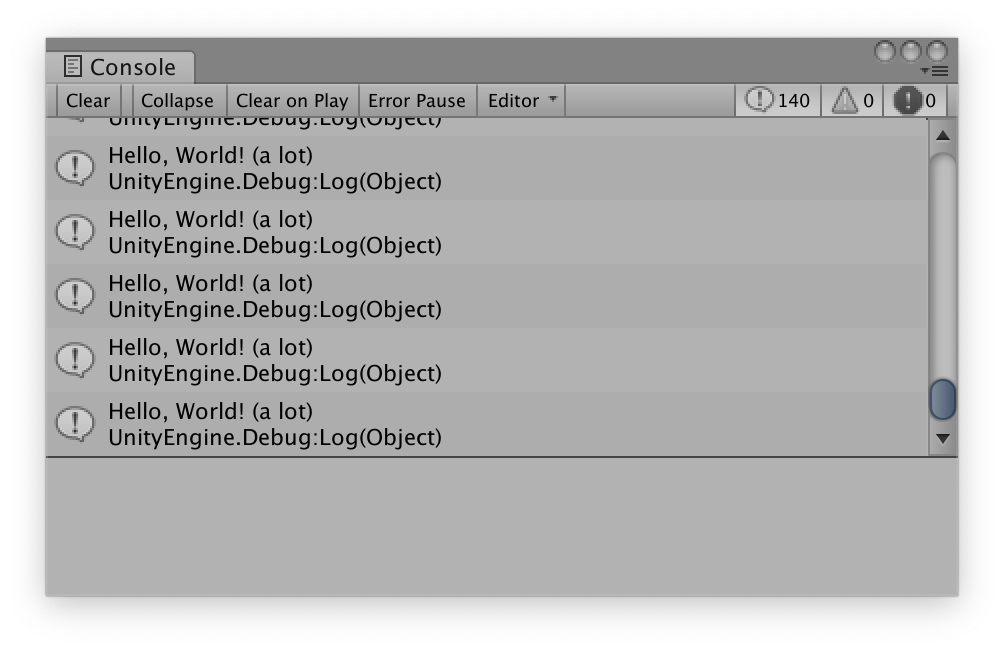
\includegraphics[width=0.45\textwidth]{collapse-1}} $\Big /$
\raisebox{-.45\height}{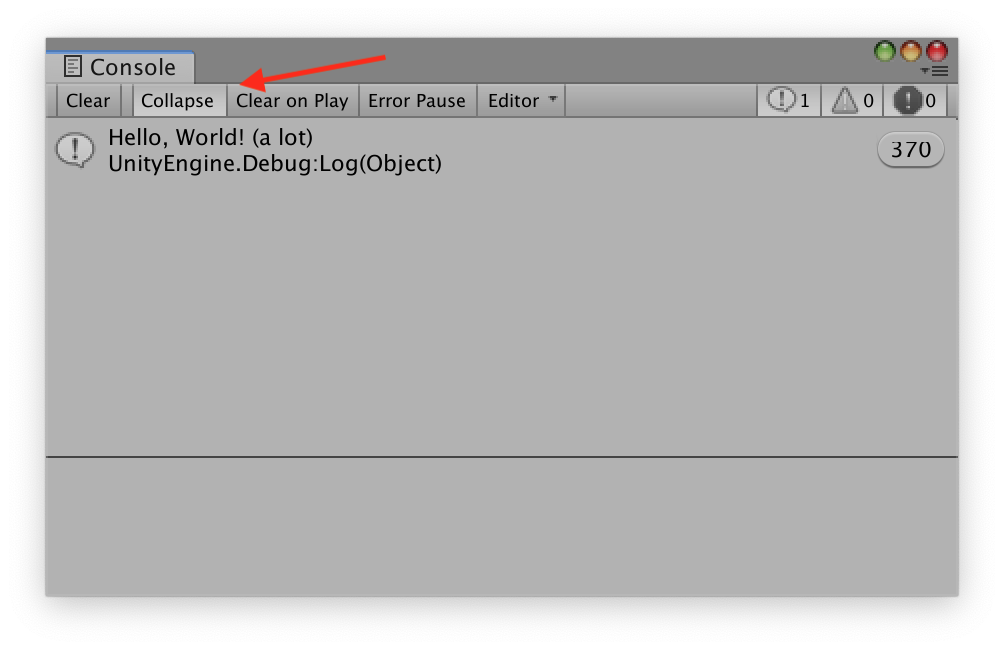
\includegraphics[width=0.45\textwidth]{collapse-2}}
\end{center}

\section{Adding Fields to Components}

You may recall that Unity's built-in components are all \textit{configurable} via the inspector.
For example, we can modify a Box Collider's extents or a Character Controller's walk speed.  You can
make your own components configurable as well.  There are two ways to do this:
\begin{enumerate}
    \item Add a \lstinline|public| variable to your component class
    \item Add a \lstinline|private| variable to your component class with \lstinline|[SerializeField]|
          before the declaration.  Special keywords in square brackets like SerializeField are called
          \textbf{attributes} in C\#.  Attributes allow you to give hints about how your code should
          be treated by the C\# compiler and Unity's runtime; you can read more on them 
          \href{https://docs.microsoft.com/en-us/dotnet/csharp/programming-guide/concepts/attributes/}{here}.
          Read more on \lstinline|[SerializeField]| in the 
          \href{https://docs.unity3d.com/ScriptReference/SerializeField.html}{Unity Scripting Reference}.
\end{enumerate}
It is a matter of style whether or not you want to use \lstinline|public| or \lstinline|[SerializedField] private|
variables; in general you should use \lstinline|public| \textit{only} if you intend for other scripts
to modify that value.  Unity will automatically detect the type of each field and add a corresponding
editor in the Unity inspector.  Below is a simple modification on the \lstinline|StartTester| that
allows for a custom String to print:

\directory{BasicFunctions/FieldTester.cs}
\StartLineAt{1}
\begin{csharp}
using UnityEngine;

public class FieldTester : MonoBehaviour
{
    // Mark fields with [SerializeField] to allow 
    // them to be edited in the inspector
    [SerializeField]
    private string StringToPrint;

    private void Start()
    {
        Debug.Log(StringToPrint);
    }
}
\end{csharp}

\begin{wrapfigure}[9]{r}[30pt]{0.5\textwidth}
    \vspace*{-2em}
    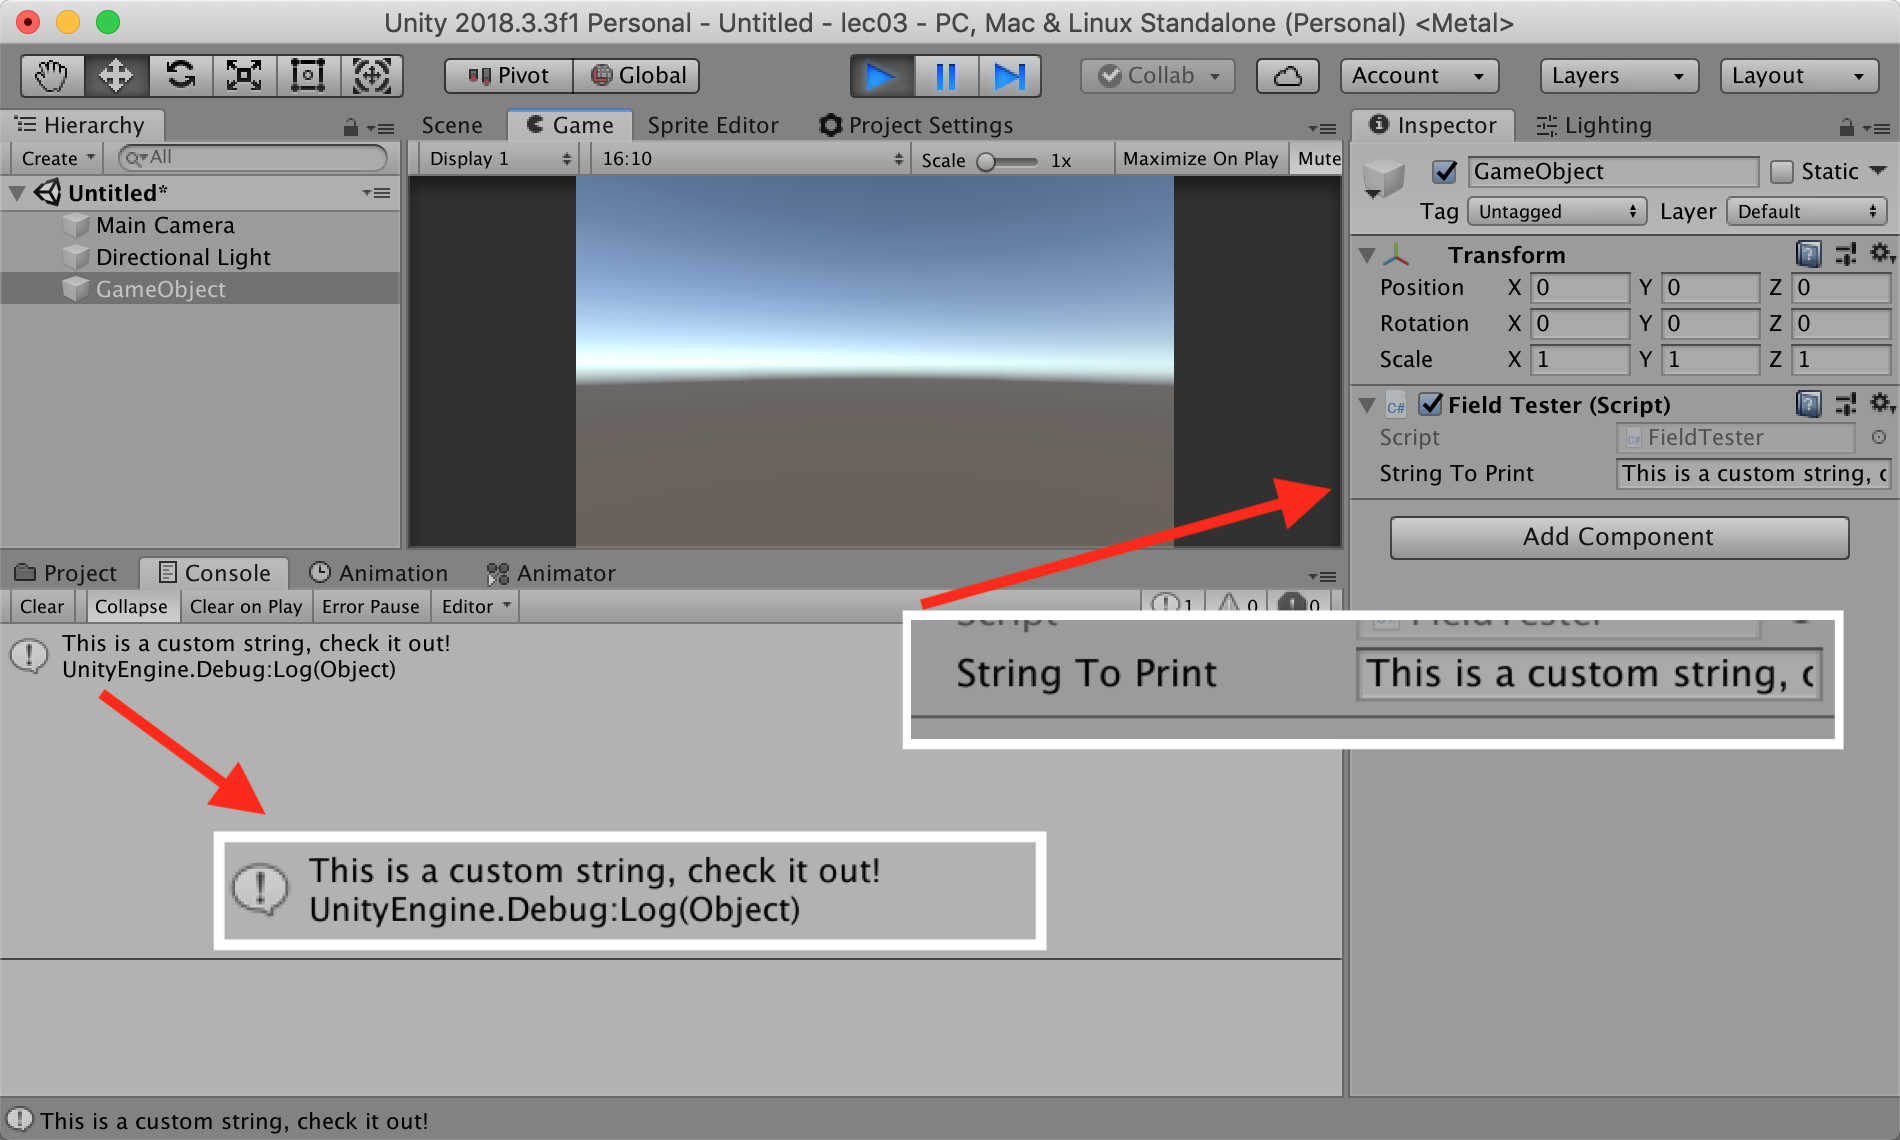
\includegraphics[width=0.5\textwidth]{fields}
\end{wrapfigure}

Here is what this script looks like in the Unity inspector:
Notice how Unity once again picked up on the camel casing of \texttt{StringToPrint} and also
detected the type of the variable (\texttt{string}).  The input field that Unity displays is
specific to this type.  In fact, many different types are supported by Unity to be displayed via
\texttt{[SerializedField]}.  These types are known as \textbf{Serializable Types} \footnote{
The term \textit{Serializable} is rooted in a C\# concept known as \textit{Serialization}.  From
the Microsoft C\# documentation: ``Serialization is the process of converting an object into a 
stream of bytes to store the object or transmit it to memory, a database, or a file.'' 
(\href{https://docs.microsoft.com/en-us/dotnet/csharp/programming-guide/concepts/serialization/index}{Source})
Unity is internally Serializing your game data to an asset file.}
Here's a summary of which types are supported (Source:
\href{https://docs.unity3d.com/ScriptReference/SerializeField.html}{Unity Scripting Reference}):

\begin{enumerate}
    \setlength\itemsep{0.25em}
    \item All classes inheriting from \lstinline|UnityEngine.Object|, for example \lstinline|GameObject|, 
          \lstinline|Component|, \lstinline|MonoBehaviour|, \lstinline|Texture2D|, 
          and \lstinline|AnimationClip|.
    \item All basic data types like \lstinline|int|, \lstinline|string|, \lstinline|float|, 
          and \lstinline|bool|.
    \item Unity types: \lstinline|Vector2|, \lstinline|Vector3|, \lstinline|Vector4|, 
          \lstinline|Quaternion|, \lstinline|Matrix4x4|, \lstinline|Color|, \lstinline|Rect|, 
          \lstinline|LayerMask|$\dots$
    \item Arrays of a serializable type (For example: \lstinline|int[]|, \lstinline|GameObject[]|)
    \item Lists of a serializable type (For example: \lstinline|List<Vector3>|)
    \item \lstinline|enum| types (more info 
    \href{https://docs.microsoft.com/en-us/dotnet/csharp/language-reference/keywords/enum}{here})
    \item \lstinline|struct|s, as well as \lstinline|class|es marked with the 
          \lstinline|[System.Serializable]| annotation.
\end{enumerate}

\noindent The next example demonstrates different types of interesting Serializable types that are 
built in to Unity:
\pagebreak

\directory{BasicFunctions/LotsOfFieldsTester.cs}

\begin{wrapfigure}[0]{r}[30pt]{0.45\textwidth}
    \vspace*{20em}
    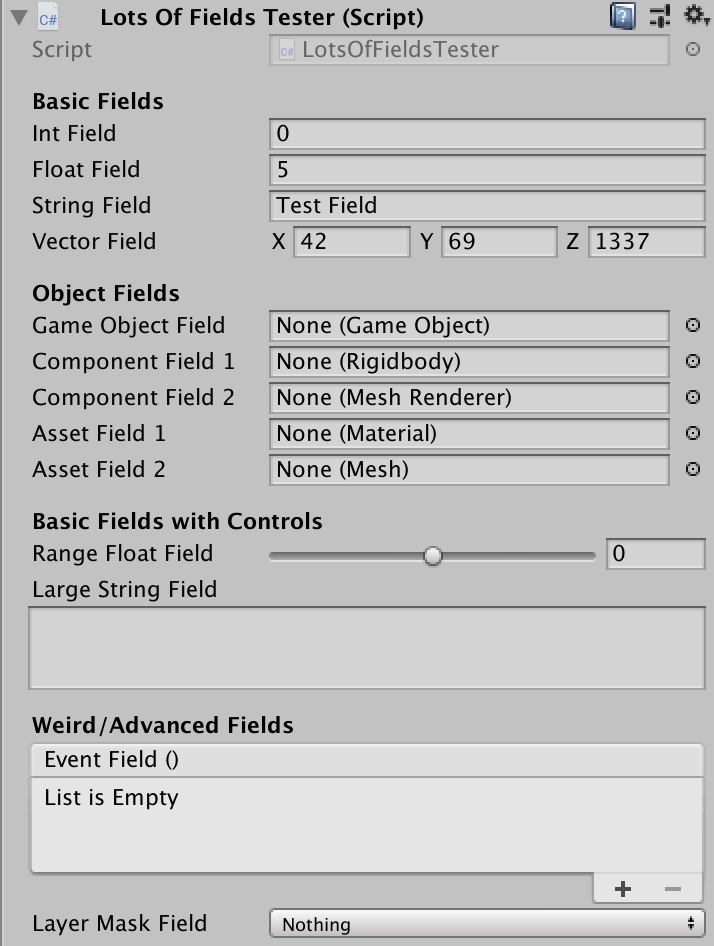
\includegraphics[width=0.45\textwidth]{lots-of-fields}
\end{wrapfigure}
\StartLineAt{1}
\begin{csharp}
using UnityEngine;
using UnityEngine.Events;

public class LotsOfFieldsTester : MonoBehaviour
{
    [Header("Basic Fields")]
    [SerializeField]
    private int _IntField;
    [SerializeField]
    private float _FloatField = 5.0f;
    [SerializeField]
    private string _StringField = "Test Field";
    [SerializeField]
    private Vector3 _VectorField = new Vector3(42, 69, 1337);

    [Header("Object Fields")]
    [SerializeField]
    private GameObject _GameObjectField;
    [SerializeField]
    private Rigidbody _ComponentField1;
    [SerializeField]
    private MeshRenderer _ComponentField2;
    [SerializeField]
    private Material _AssetField1;
    [SerializeField]
    private Mesh _AssetField2;

    [Header("Basic Fields with Controls")]
    [SerializeField]
    [Range(-1.0f, 1.0f)]
    private float _RangeFloatField;
    [SerializeField]
    [TextArea]
    private string _LargeStringField;
    [Header("Weird/Advanced Fields")]
    [SerializeField]
    private UnityEvent _EventField;
    [SerializeField]
    private LayerMask _LayerMaskField;
}
\end{csharp}

Importantly, we can create fields for the basic types (\lstinline|float|, \lstinline|Vector3|, etc)
but also for complex Unity types (components like \lstinline|MeshRenderer|, GameObjects, Materials$\dots$).
Also here I use the \lstinline|[Header(string)]| attribute to add a nice bold header before certain
controls.  This is for aesthetic purposes only and does not affect gameplay, but can be nice to
organize your fields for level designers.  To set a default value, simply set the variable in your
script equal to something (see the \lstinline|_VectorField| for example)

\section{Procedural Animation}

One of the most common tasks that you need to do when creating components is to move GameObjects.
The \lstinline|transform| variable, available to all \lstinline|MonoBehaviour|s, allows you to change
the position, rotation, scale, and parent of any GameObject.  For example, \lstinline|transform.position = Vector3.zero;|
translates the current script's GameObject to the origin (\lstinline|Vector3|s are used to represent
any kind of X/Y/Z position).  The globally-accessible constant \lstinline|Time.time| gives you the
current time, in seconds, since the game launched.  You can use this to build simple animations:

\directory{BasicFunctions/ClosedFormAnimation.cs}
\StartLineAt{1}
\begin{csharp}
using UnityEngine;

public class ClosedFormAnimation : MonoBehaviour
{
    [SerializeField]
    private float Radius = 1.0f;
    [SerializeField]
    // Vector3.zero == new Vector3(0,0,0)
    private Vector3 Center = Vector3.zero;
    [SerializeField]
    private float Speed = 1.0f;

    private void Update()
    {
        float s = Mathf.Sin(Time.time * Speed);
        float c = Mathf.Cos(Time.time * Speed);

        transform.position = Center + new Vector3(c * Radius, s * Radius, 0);
    }
}
\end{csharp}

The above script moves the GameObject it is attached to in a circle.  The radius and center of the 
circle are given by variables in the inspector, as well as the speed of movement in radians per 
second.  We use the Unity-provided \href{https://docs.unity3d.com/ScriptReference/Mathf.html}{Mathf}
library to get \lstinline|Sin| and \lstinline|Cos| functions, which are used to calculate the final
position using basic trigonometry.  Importantly, we use \lstinline|Time.time| to find the position
along the circle.

In real games, however, your components need to \textit{respond} to ``stimuli'' that are outside of
your control.  For example, you may need to respond to user input which is totally unpredictable.
Because of this, using \lstinline|Time.time| to calculate an absolute position won't cut it.  Instead,
we would like to control the \textit{velocity} of the parent GameObject over time.  The below script
is an example of this concept: instead of \textit{setting} the position explicitly, we are \textit{adding}
to the ``current'' position.\pagebreak

\directory{BasicFunctions/DeltaTimeAnimation.cs}
\StartLineAt{1}
\begin{csharp}
using UnityEngine;

public class DeltaTimeAnimation : MonoBehaviour
{
    public float Speed = 1.0f; // speed in m/s
    public Vector3 Direction = new Vector3(1,0,0);
    public bool localPosition = false;

    // Update is called once per frame
    private void Update()
    {
        Vector3 delta = Speed * Direction.normalized * Time.deltaTime;

        if (localPosition)
            transform.localPosition += delta;
        else
            transform.position += delta;
    }
}
\end{csharp}

\lstinline|Time.deltaTime| gives the time in seconds \textit{since the last call to Update()}.  It is
used here on line 12 to ensure that the movement speed is independent of framerate.  Let's say, for
example, that you set the speed variable to 1 m/s.  If you didn't multiply by \lstinline|Time.deltaTime|,
then assuming 60fps you would be moving at around 60 m/s!  Even more worryingly, the GameObject would
move faster on faster machines.  Another way of thinking of this is via dimensional analysis;
\lstinline|Speed| is in $\frac{\mathrm{m}}{\mathrm{s}}$ and we want to know how many meters to move.  
By multiplying by \lstinline|Time.deltaTime|, which is measured in seconds, we have
$\frac{\mathrm{m}}{\mathrm{s}} \times \mathrm{s} = \mathrm{m}$, which is what we want.  Also highlighted
here is the difference between \lstinline|transform.position| and \lstinline|transform.localPosition|.
\lstinline|transform.position| changes the \textit{absolute} position of the GameObject, ignoring
any parenting.  \lstinline|transform.localPosition| represents the position of the GameObject
\textit{relative to} the parent GameObject (if the transform has no parent, the two values are the same).

\subsection{Responding to User Input}

\begin{wrapfigure}[10]{r}[30pt]{0.45\textwidth}
    \vspace*{-3.5em}
    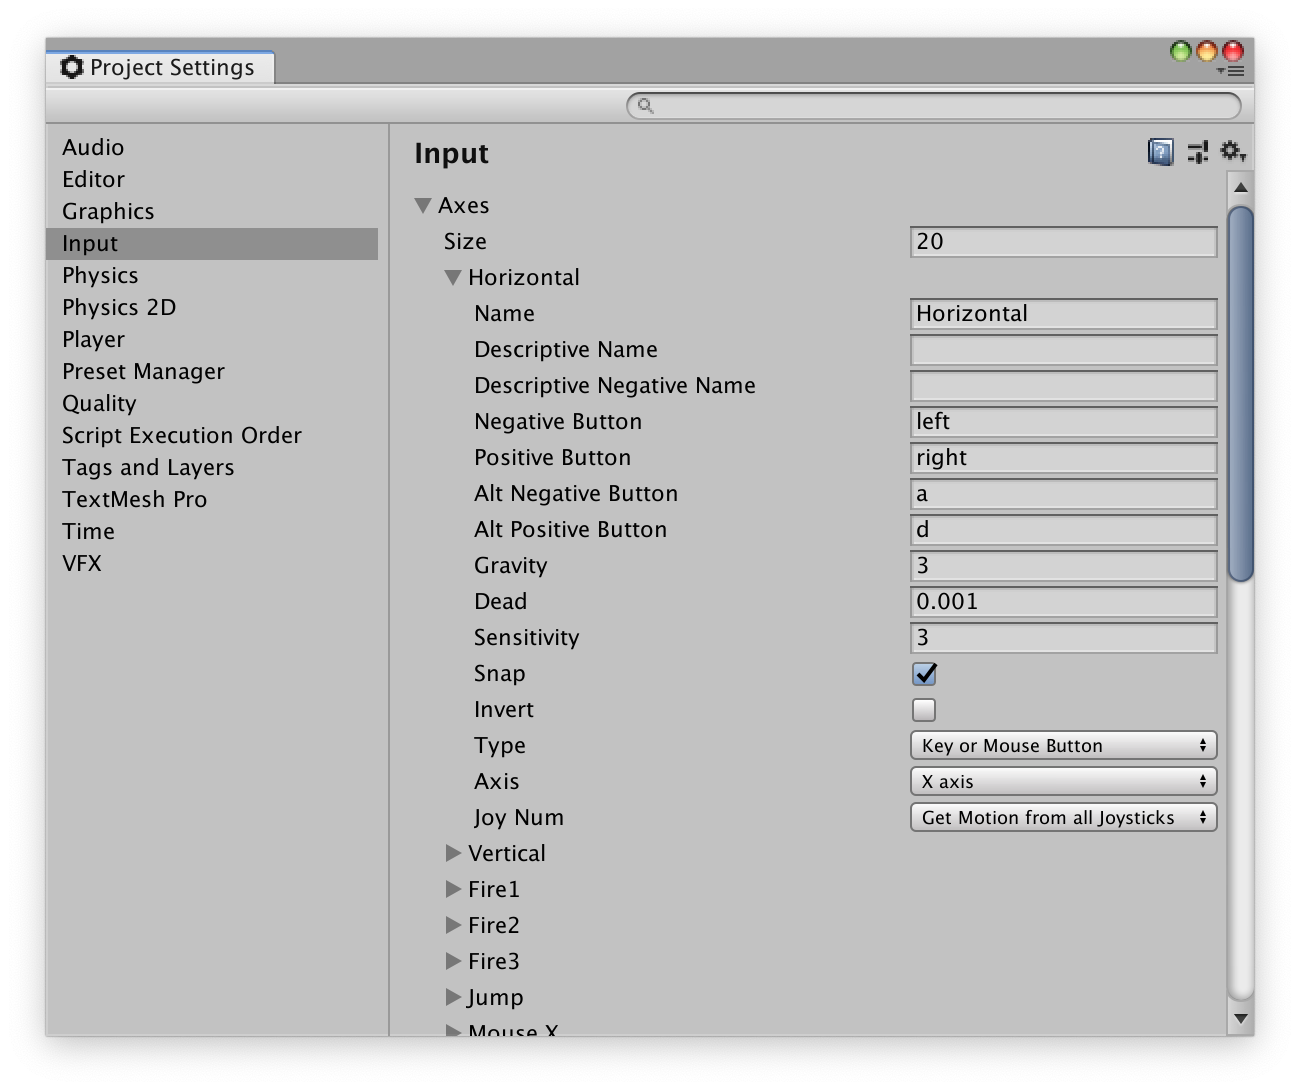
\includegraphics[width=0.45\textwidth]{input-manager}
\end{wrapfigure}
One common task when building a game is to respond to some input by the player.  This could be
the Mouse, Keyboard, or a Gamepad.  Unity requires that all \textit{possible} inputs are first
outlined in the \textbf{Input Manager}.  Open the input manager via \menu{Edit>Project Settings$\dots$}
and select the \menu{Input} submenu.  The input manager consists of a set of named \textbf{Input Axes}
that list out all of the possible inputs to your game.  The default set of inputs, shown to the right,
cover most common inputs that you would need in a simple game.  For example, the ``Horizontal'' axis
sets the so-called \textit{positive button} to \keys{\arrowkey{>}} / \keys{D} and the \textit{negative
button} to \keys{\arrowkey{<}} / \keys{A}.  If you scroll down the input manager, you will find a
second entry for ``Horizontal'' that is configured to respond to the X axis of a joystick.  What this
means is that the ``Horizontal'' axis will have a value of $-1$ if you press \keys{\arrowkey{<}} / \keys{A}
or if you hold the left stick on a gamepad to the left, and it will have a value of $+1$ if you press
\keys{\arrowkey{>}} / \keys{D} or hold the left stick on a gamepad to the right.  You can read more
about each option in the Input Manager in the \href{https://docs.unity3d.com/Manual/class-InputManager.html}{Unity Manual here}.

The next script shows how to access these input axis values from within \lstinline|Update()|.  The
operative command is \lstinline|Input.GetAxis(string)|, which returns a \lstinline|float| -- usually
ranging from $-1$ to $+1$ -- of the value at that axis.  The parameter matches the name of each axis
that we configured in the Input Manager: in this case ``Horizontal'' and ``Vertical.''  I like to
allow the axis names to be configurable in Unity, so that if we need to change the Input Manager
then we don't need to dive in to each script to fix the axis names.

\directory{BasicFunctions/SimpleMovement.cs}
\StartLineAt{1}
\begin{csharp}
using UnityEngine;

public class SimpleMovement : MonoBehaviour
{
    [SerializeField]
    private string _HorizontalMovementAxis = "Horizontal";
    [SerializeField]
    private string _VerticalMovementAxis = "Vertical";
    [SerializeField]
    private float _MovementSpeed = 1.0f;

    private void Update()
    {
        float hoz = Input.GetAxis(_HorizontalMovementAxis);
        float vrt = Input.GetAxis(_VerticalMovementAxis);

        Vector3 mov = new Vector3(hoz, vrt, 0);

        if (mov.sqrMagnitude > 1.0f)
            mov.Normalize(); // make vector have length 1

        transform.position += mov * _MovementSpeed * Time.deltaTime;
    }
}
\end{csharp}

\noindent Once we have the input values (stored, again, in the range $-1 \leftrightarrow +1$ in the 
\lstinline|hoz| / \lstinline|vrt| variables) we convert them into a \lstinline|Vector3| on line 17.
On line 19, we protect against the case where the player holds both \keys{\arrowkey{>}+\arrowkey{^}}
for example.  In this case, $\texttt{hoz} = \texttt{vrt} = 1$, so the length of \texttt{mov} is
(by pythagorean theorem) $\sqrt{1^2 + 1^2} = \sqrt{2}$, which is greater than 1.  This would mean
that the player can move faster by moving diagonally!  This bug is actually pretty common in games
with 2D movement (especially bad console ports).  The solution is to call \lstinline|mov.Normalize()|,
which replaces \lstinline|mov| with a vector in the same direction, but with length 1.  If you attach
\lstinline|SimpleMovement.cs| to a GameObject, you can now control it with the arrow keys
(or any other of the keys mentioned above.)

\subsection{Accessing Other Components}

What do you do if you want to access another component of the current GameObject?  For example, our
script might want to change the movement speed of a player character, the color of an object, etc.
You can use the \lstinline|GetComponent<Type>()| function (available to all \lstinline|MonoBehaviour|s)
to access the component attached to the same GameObject as the caller with type \lstinline|Type|.
The following example illustrates how to use \lstinline|GetComponent| to change the color of a
GameObject.  To do this we need to modify the GameObject's Material, which is stored in the
\textit{Mesh Renderer} component (as seen in lecture 2).  Unity's components are named after the class
names in C\# scripts, just like your own components.  Therefore we can deduce that the C\# type
of the ``Mesh Renderer'' component is \lstinline|MeshRenderer|.  Similarly ``Box Collider'' has
the type \lstinline|BoxCollider|, ``Rigidbody 2D'' has type \lstinline|Rigidbody2D|, etc.

\directory{BasicFunctions/ChangeMaterialTester.cs}
\StartLineAt{1}
\begin{csharp}
using UnityEngine;

[RequireComponent(typeof(MeshRenderer))]
public class ChangeMaterialTester : MonoBehaviour
{
    [SerializeField]
    private Gradient _Gradient;
    [SerializeField]
    [Tooltip("Length in seconds to cycle through the gradient")]
    private float _CycleLength;

    // Note: This field isn't serialized, so we can't edit it in the inspector!
    private MeshRenderer _Renderer;

    private void Start()
    {
        // GetComponent<T> gets the component
        // with type T attached to the current GameObject.
        // If none exist, returns null
        _Renderer = GetComponent<MeshRenderer>();
    }

    private void Update()
    {
        float a = (Mathf.Cos(Time.time / _CycleLength * (2.0f * Mathf.PI)) + 1.0f) / 2.0f;
        Color c = _Gradient.Evaluate(a);

        // _Renderer.material has type `Material`
        // Material.color has type `Color`
        _Renderer.material.color = c;
    }
}
\end{csharp}

This example also makes use of the built-in \lstinline|Gradient| type to cycle between many colors
over time.  The value \lstinline|float a| in \lstinline|Update| cycles from 0 to 1 as time moves 
forward, and the gradient is \textit{evaluated} at that value.  The \lstinline|Color| type is used 
to represent RGBA color values; we get at our \lstinline|MeshRenderer|'s material via
\lstinline|MeshRenderer.material| and further are able to change the color via \lstinline|Material.color|.
How do I know all of this?  Am I a god, and have just memorized all of the keywords?  Of course not:
I simply went to Unity's \textbf{Scripting Reference}, which can be accessed at
\begin{center}\href{https://docs.unity3d.com/ScriptReference}{https://docs.unity3d.com/ScriptReference}\end{center}

For example, you can find a reference for the \lstinline|MeshRenderer| 
\href{https://docs.unity3d.com/ScriptReference/MeshRenderer.html}{here} and a reference for
\lstinline|Gradient| \href{https://docs.unity3d.com/ScriptReference/Gradient.html}{here}.  The
Scripting API reference pages are an \textit{absolutely essential reference} for Unity programmers--if
you want to learn all of Unity's ins and outs, expect to look at this often!  Anyway, here's what
this script looks like in the inspector.  The Gradient type happens to have a really awesome interactive editor:

\begin{center}
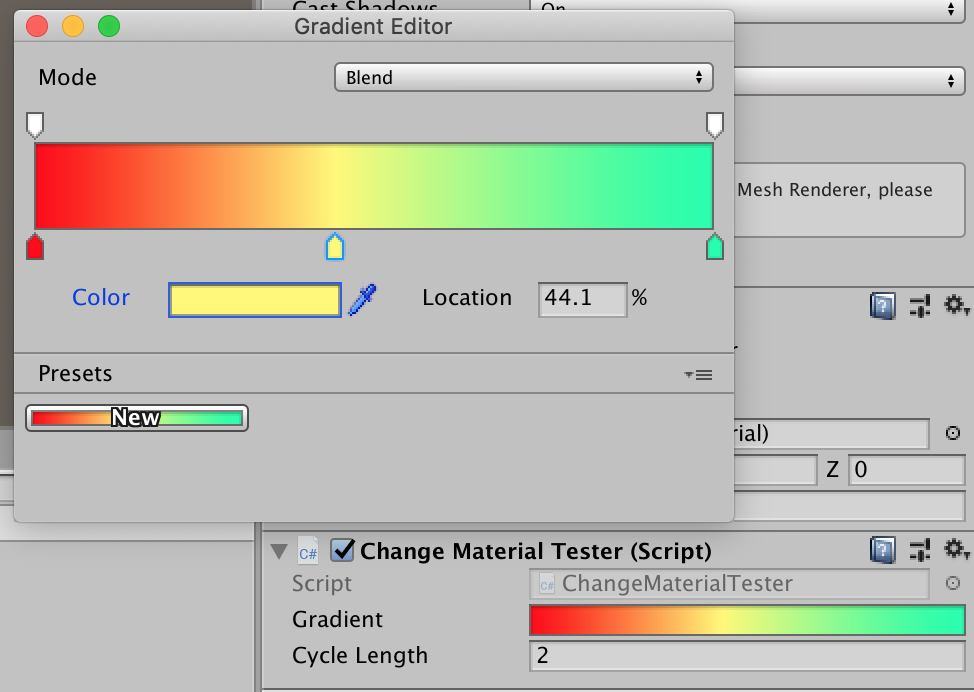
\includegraphics[height=15em]{gradient-1}\\
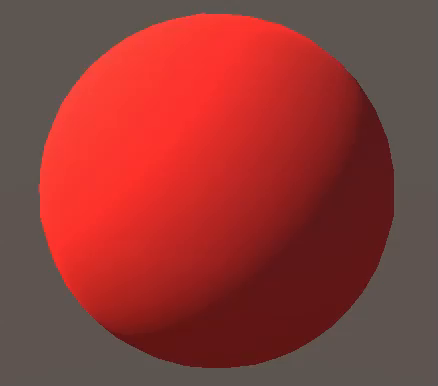
\includegraphics[height=4em]{gradient-display-0}
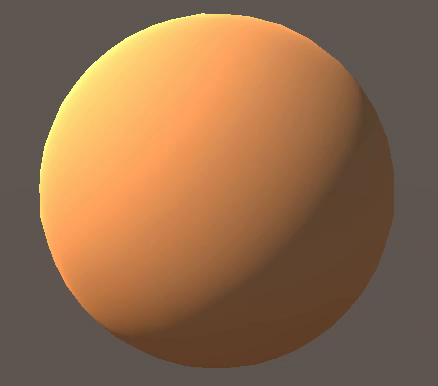
\includegraphics[height=4em]{gradient-display-1}
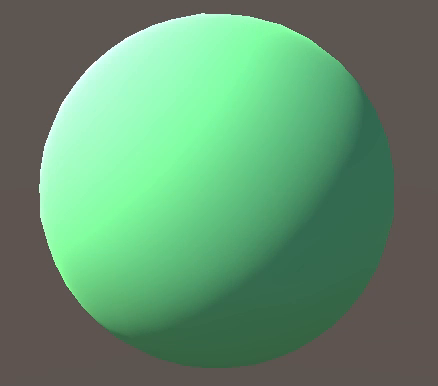
\includegraphics[height=4em]{gradient-display-2}
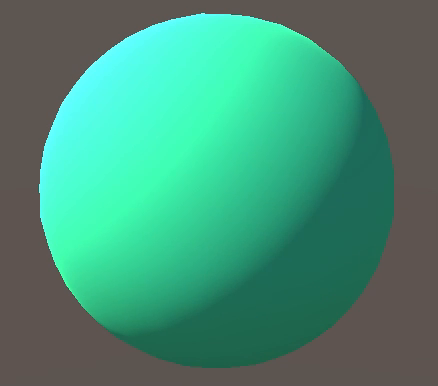
\includegraphics[height=4em]{gradient-display-3}
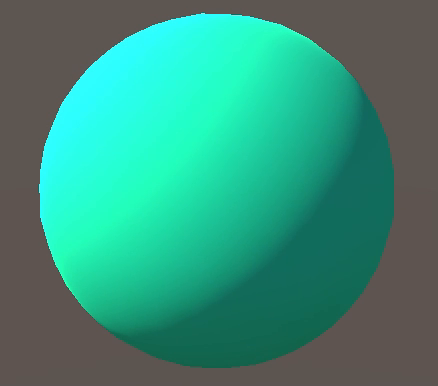
\includegraphics[height=4em]{gradient-display-4}
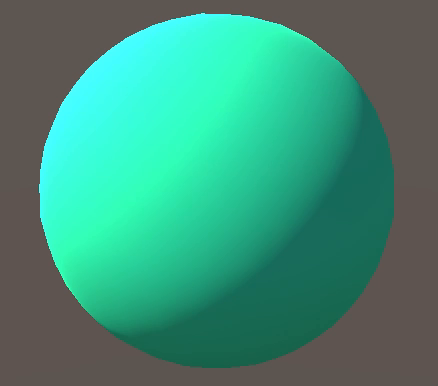
\includegraphics[height=4em]{gradient-display-5}\\
Top: The gradient popup menu featured in \lstinline|ChangeMaterialTester|.\\
Bottom: Result when attached to a sphere.
\end{center}

\section{Talking to the Physics Engine}

At one point when making almost any game, you'll have to deal with \underline{collisions}.  You need
to think about collisions when a projectile leaves a cannon, a pong ball bounces off the paddle, 
Mario hits the bottom of an item box, Sonic collects a ring, etc.  In many cases, you want to
\textit{react} to collisions (for example: when the player collides with a coin GameObject you
might want to destroy the coin, spawn a shiny particle effect, and increment a coin counter).
In the last lecture, we talked about \textbf{Colliders}.  Colliders are special components that
talk with Unity's physics engine and mark a GameObject as ``collidable.''  You also use Colliders
to define the \textit{shape} of the collidable object (which can be different than what is rendered
on screen).  There are a few different types of colliders: the \textit{Box Collider} and \textit{Sphere Collider}
are shaped like a Box and Sphere, and the \textit{Mesh Collider} allows you to specify a mesh to collide
with.  As we discussed in the last lecture, you can additionally add a \textit{Rigidbody} component
to have Unity simulate the GameObject, applying forces such as Gravity and reacting to collisions
realistically.

If you want to respond to collisions with your own logic, create a C\# script as normal.  Instead
of using \lstinline|Start| or \lstinline|Update| to check for collisions, we can use the built-in
\lstinline|OnCollisionEnter| / \lstinline|OnCollisionExit| / \lstinline|OnTriggerEnter| / 
\lstinline|OnTriggerExit| functions.  Recall from the last lecture that \textit{triggers} are
colliders with the ``Is Trigger'' option enabled in the inspector.  Triggers do not affect GameObjects
physically (for example they don't block rigidbodies from overlapping with them).  Instead, triggers are meant
to be used by your scripts for logic.  For example, in a Mario game you would want to set the coins
as triggers so that they do not affect Mario's velocity when you collect them.  However you would want
to set the item boxes as Colliders because Mario should be able to bump his head against them.

\directory{PhysicsExamples/CollisionDetectionTester.cs}
\StartLineAt{1}
\begin{csharp}
using UnityEngine;

public class CollisionDetectionTester : MonoBehaviour
{
    private void OnTriggerEnter(Collider other)
    {
        Debug.Log(gameObject.name + " just got triggered by " + other.gameObject.name);
    }

    private void OnTriggerExit(Collider other)
    {
        Debug.Log(gameObject.name + " just ended trigger by " + other.gameObject.name);
    }

    private void OnCollisionEnter(Collision collision)
    {
        Debug.Log(gameObject.name + " just collided with " + collision.gameObject.name);
    }

    private void OnCollisionExit(Collision collision)
    {
        Debug.Log(gameObject.name + " just ended collision with " + collision.gameObject.name);
    }
}
\end{csharp}

To demonstrate this script, below is a scene with three cubes.  The bottom cube, called ``Ground,''
has a Box Collider with \textit{Is Trigger} \underline{disabled}.  The middle (transparent green) cube,
named ``Trigger,'' has a Box Collider with \textit{Is Trigger} \underline{enabled}.  The top cube, named ``Falling
Cube,'' has a Box Collider and a Rigidbody attached.  The ground and trigger cubes both have the above
\lstinline|CollisionDetectionTester| component.  When we run the script, \lstinline|OnTriger{Enter,Exit}|
is called on the trigger when the falling cube enters and exits it, and \lstinline|OnCollisisonEnter| 
is called on the ground when the falling cube collides with it.  Because the falling cube never
stops colliding with the ground, \lstinline|OnCollisionExit| is not called.

\begin{center}
\raisebox{-.45\height}{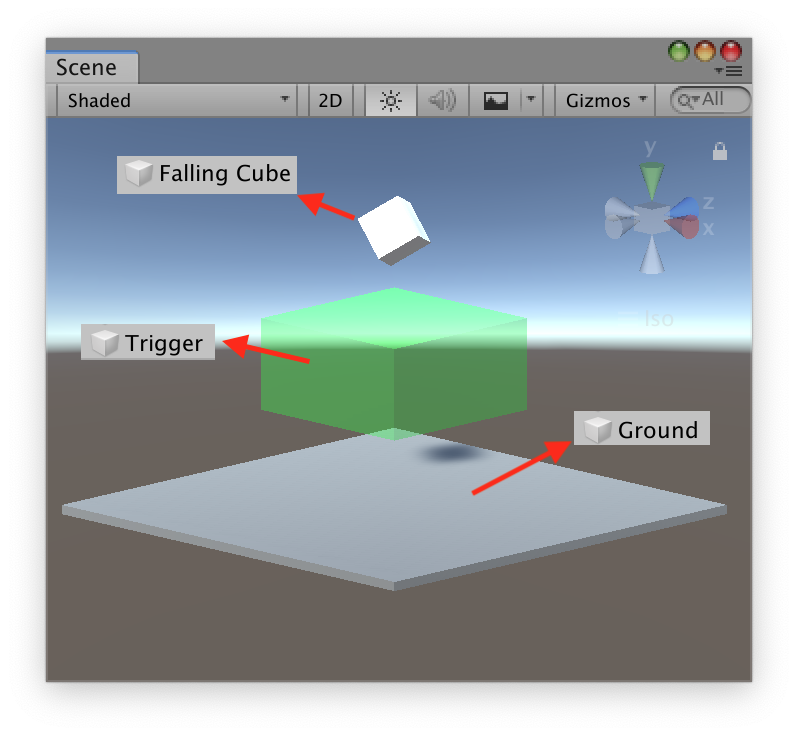
\includegraphics[height=12em]{collision-1}} $\rightarrow$
\raisebox{-.45\height}{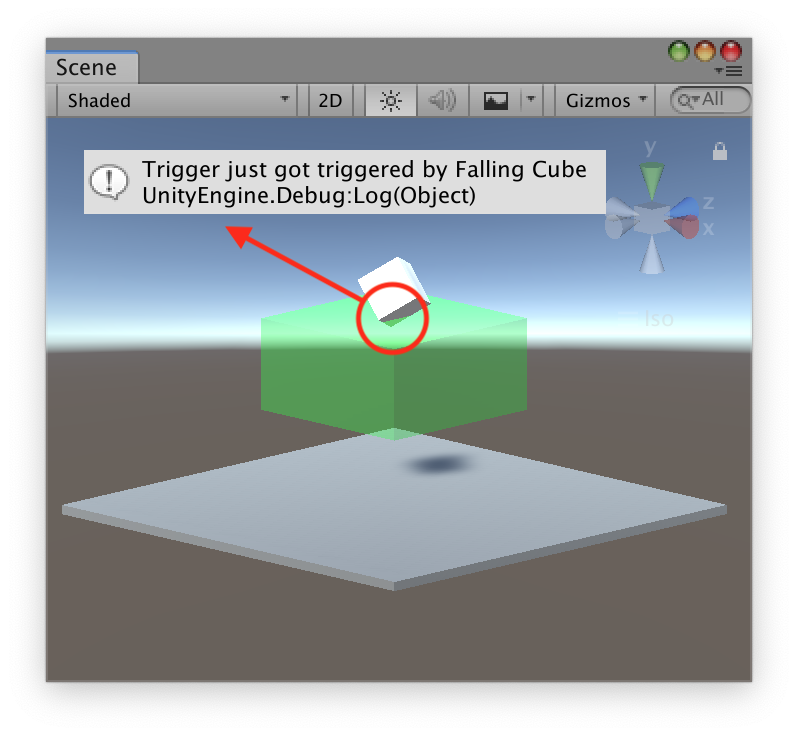
\includegraphics[height=12em]{collision-2}} $\rightarrow$
\raisebox{-.45\height}{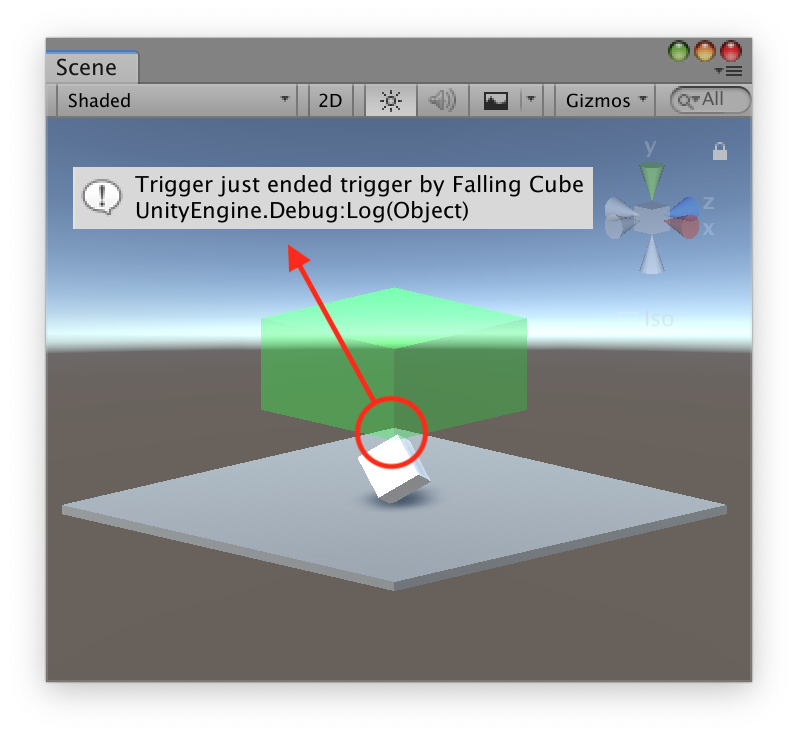
\includegraphics[height=12em]{collision-3}} $\rightarrow$
\raisebox{-.45\height}{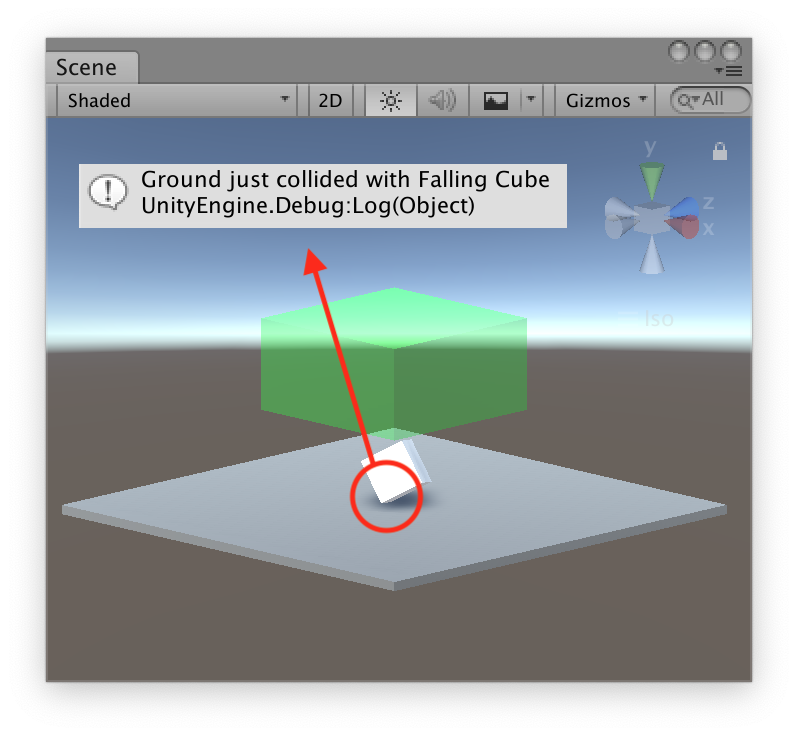
\includegraphics[height=12em]{collision-4}} $\rightarrow$
\raisebox{-.45\height}{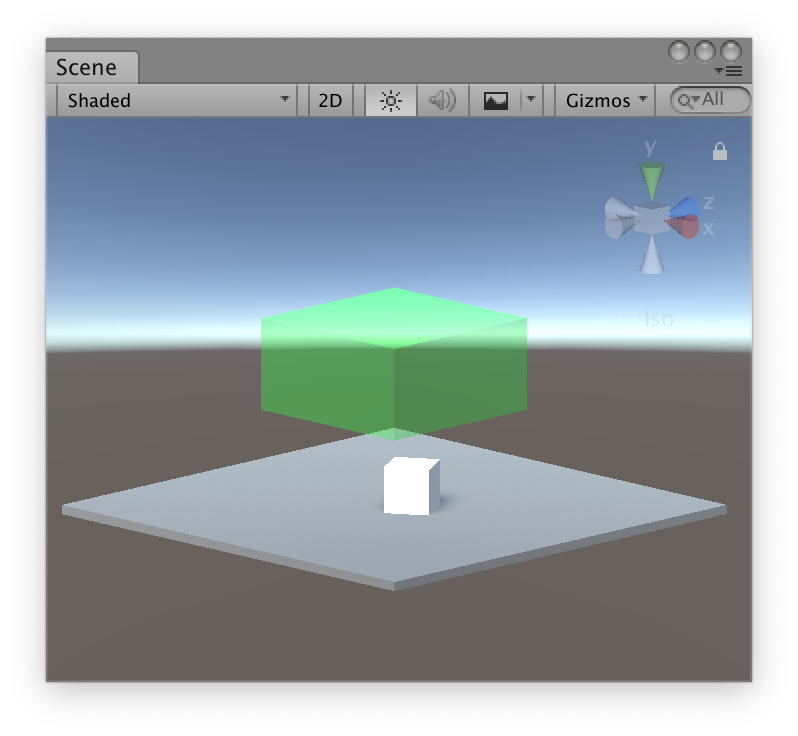
\includegraphics[height=12em]{collision-5}}
\end{center}

This is also the first time that I've used the \lstinline|gameObject| variable.  \lstinline|gameObject|
is available to all \lstinline|MonoBehaviour|s and provides a pointer to the ``owner'' of this instance
of the \lstinline|MonoBehaviour|.  The type of \lstinline|gameObject| is 
\href{https://docs.unity3d.com/ScriptReference/GameObject.html}{\lstinline|UnityEngine.GameObject|}.

If you are making a 2D game, there is a completely different set of components that you need to use
for Physics.  For example, in a 2D game, instead of using a \textit{Box Collider} component you should
use a \textit{Box Collider 2D}.  There is a 2D version of every physics component: \textit{Rigidbody}
and \textit{Rigidbody 2D}, \textit{Sphere Collider} and \textit{Circle Collider 2D}, etc.  Similarly,
when responding to 2D collision we need to use 2D variants of the collision response functions:
\lstinline|OnTriggerEnter2D|, \lstinline|OnTriggerExit2D|, \lstinline|OnCollisionEnter2D|,
\lstinline|OnCollisionExit2D|.  Unity is built this way because under the hood, the 3D physics system
uses \href{https://www.geforce.com/hardware/technology/physx}{NVIDIA PhysX}, which is optimized for
3D games.  The 2D physics system uses the \href{https://github.com/erincatto/box2d}{Box2D Physics Engine},
which is purpose-built for 2D games.  On the next page is a 2D variant of the collision detection 
tester that will respond to 2D physics components.  \textbf{Do not use the 3D versions of 
OnCollision/OnTrigger functions with 2D colliders!}\pagebreak

\directory{PhysicsExamples/CollisionDetectionTester2D.cs}
\StartLineAt{1}
\begin{csharp}
using UnityEngine;

public class CollisionDetectionTester2D : MonoBehaviour
{
    private void OnTriggerEnter2D(Collider2D other)
    {
        Debug.Log("Just got triggered by GameObject called " + other.gameObject.name);
    }

    private void OnTriggerExit2D(Collider2D other)
    {
        Debug.Log("Just ended trigger by GameObject called " + other.gameObject.name);
    }

    private void OnCollisionEnter2D(Collision2D collision)
    {
        Debug.Log("Just collided with GameObject called " + collision.gameObject.name);
    }

    private void OnCollisionExit2D(Collision2D collision)
    {
        Debug.Log("Just ended collision with GameObject called " + collision.gameObject.name);
    }
}
\end{csharp}

\section{Using UnityEvents}

Triggers are a great opportunity to talk about a very useful feature of Unity's scripting called
\textbf{UnityEvents}.  UnityEvents are similar to \lstinline|event|s in C\# and function pointers 
in C/C++.  They are an implementation of the 
\href{http://gameprogrammingpatterns.com/command.html}{Command Design Pattern}, which is sort of like
a \textit{callback}.  UnityEvents allow you to \textit{store an \underline{action} into a
variable, such that you can execute that action at any time}.  Even better, these actions are editable
in the inspector, just like any other field!

The next script is an example of how to use UnityEvents to build Game Logic directly in the 
inspector.  We have two editable \lstinline|UnityEvent|s that are meant to respond to trigger
enter and exit events.  In the \lstinline|OnTrigger| events, we then call \lstinline|UnityEvent.Invoke()|,
which actually executes the event.  Note that if no actions are assigned to either UnityEvent,
they are set to \lstinline|null|.  So we need to check for \lstinline|null| before calling 
\lstinline|Invoke()|.\\

\directory{PhysicsExamples/EventOnTrigger.cs}
\StartLineAt{1}
\begin{csharp}
using UnityEngine;
using UnityEngine.Events; // Required for UnityEvent type

public class EventOnTrigger : MonoBehaviour
{
    [SerializeField]
    private UnityEvent _OnEnter;
    [SerializeField]
    private UnityEvent _OnExit;

    private void OnTriggerEnter(Collider other)
    {
        if(_OnEnter != null)
            _OnEnter.Invoke();
    }

    private void OnTriggerExit(Collider other)
    {
        if(_OnExit != null)
            _OnExit.Invoke();
    }
}
\end{csharp}

To demonstrate this I've set up two lights, a red and blue light.  I'd like to enable the red light
when a trigger is being triggered, and blue when it is not.  I can use the \lstinline|EventOnTrigger|
script to do this.  UnityEvents have an interactive editor in the inspector that allows you to select
which function you want to call on which GameObject.  Here I call the function 
\href{https://docs.unity3d.com/ScriptReference/GameObject.SetActive.html}{\lstinline|GameObject.SetActive()|}
to enable and disable the red and blue lights in response to each event.  Normally this would have
required me to write a new script, but UnityEvents let me do this right in the inspector!  UnityEvents
are a powerful tool, and allow you to build simple behaviors without touching a line of code.

\begin{center}
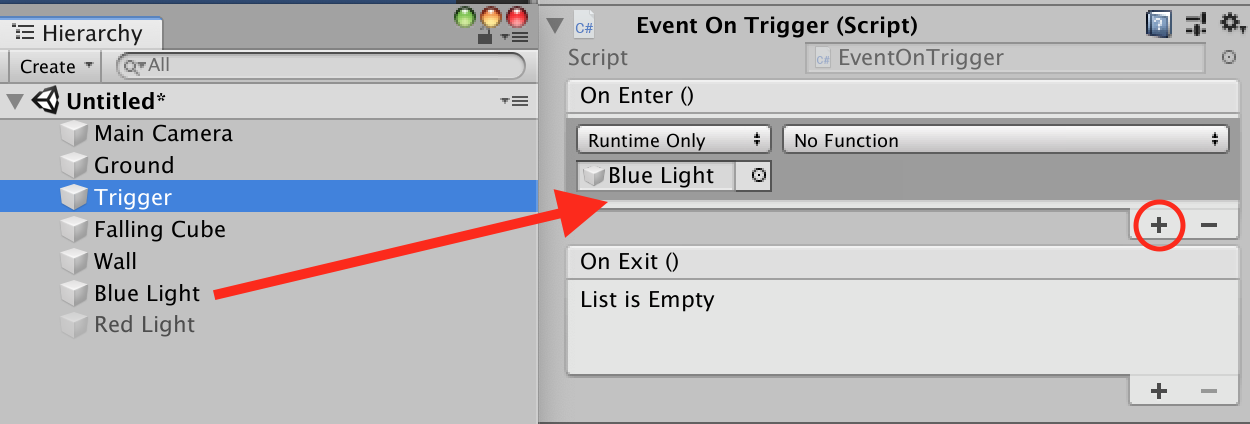
\includegraphics[height=12em]{unityevent-1} \\
Click on the \faPlus\ button to add a new action to the UnityEvent.  All actions are executed 
simultaneously upon calling \lstinline|UnityEvent.Invoke()| in your script.\\
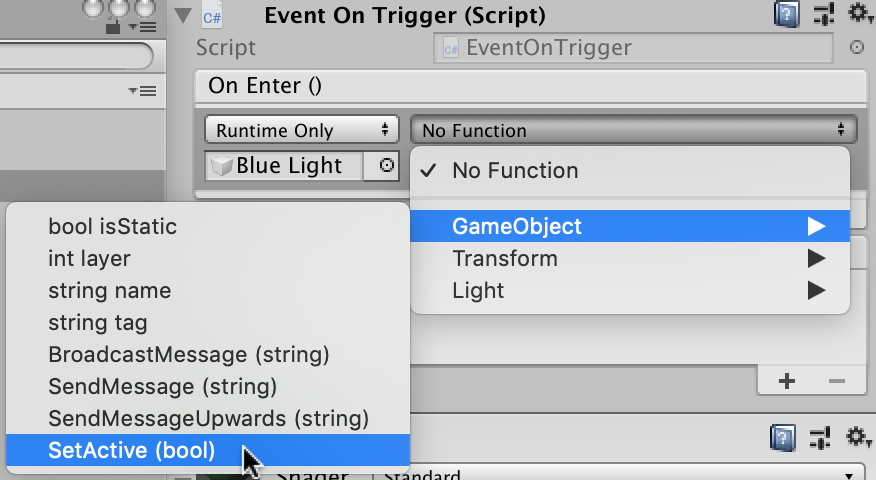
\includegraphics[height=12em]{unityevent-2} 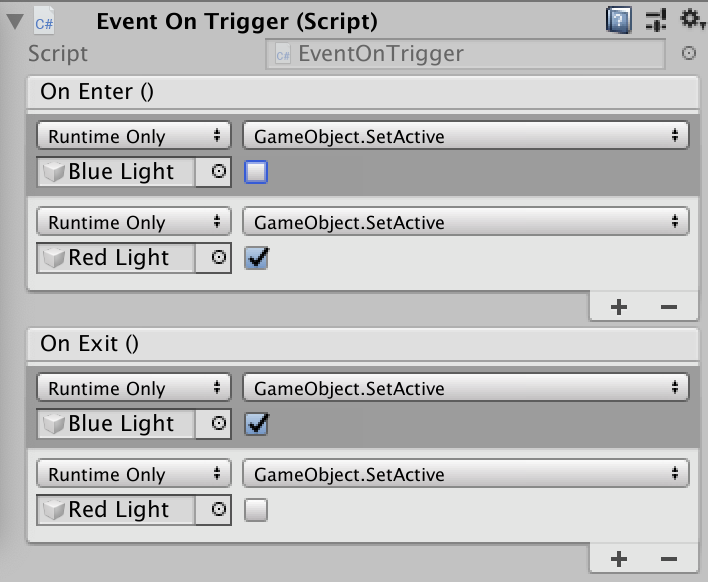
\includegraphics[height=12em]{unityevent-3} \\
Here we configure the event to enable and disable the lights.  You need to specify a \textit{target}
GameObject to call something on.  Here we are calling \lstinline{GameObject.SetActive}, but we can
call functions in the target's \lstinline|GameObject|, \lstinline|Transform|, or any component.  \\
\raisebox{-.45\height}{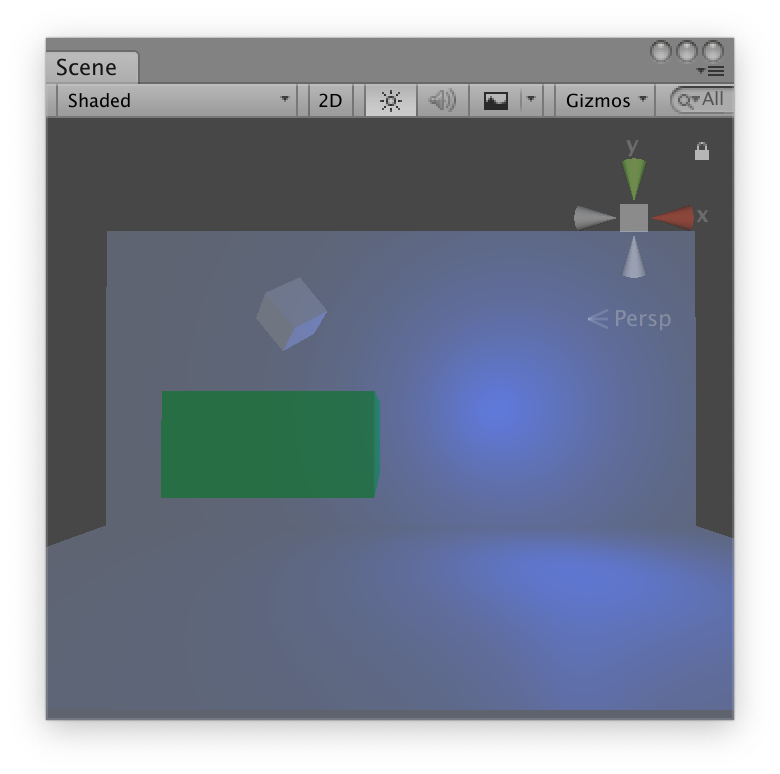
\includegraphics[height=12em]{unityevent-4}} $\rightarrow$
\raisebox{-.45\height}{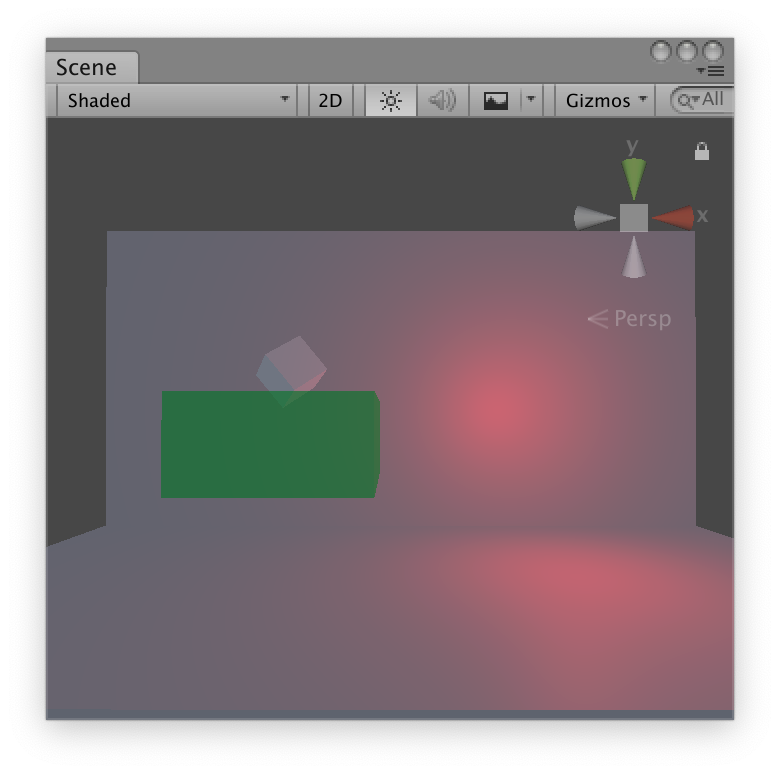
\includegraphics[height=12em]{unityevent-5}} $\rightarrow$
\raisebox{-.45\height}{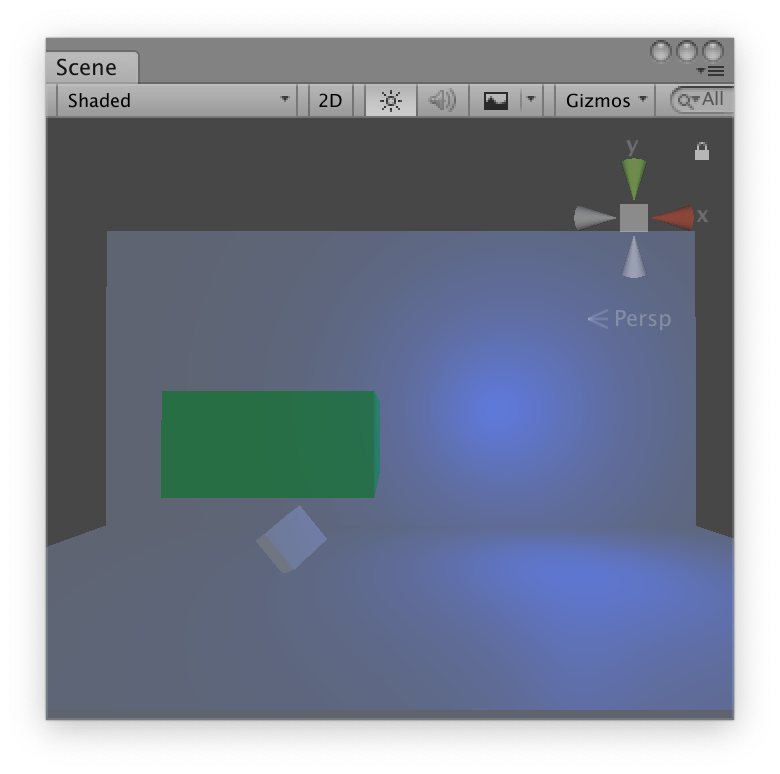
\includegraphics[height=12em]{unityevent-6}} \\
When a cube activates the trigger (the green cube), the lights are enabled and disabled as expected.
\end{center}

\section{Prefabs}

Game worlds tend to have many objects that are repeated very often.  For example, you might need
to spawn in dozens of the exact same enemy in a level.  Obviously you wouldn't want to rebuild the
enemy GameObject every time you wanted to spawn it in.  One way to solve this issue is to build the
enemy once and duplicate it (\keys{\cmd\ or Ctrl+D}).  This works at first, but what if you want to 
change a detail of your enemy after duplicating them?  You would have to re-do your change for each
instance.

Unity addresses this common problem via \textbf{Prefabs}.  Prefabs are \textit{GameObjects that are
saved to a file}.  You can create a prefab by dragging a GameObject from the hierarchy view onto the
project view.  To see prefabs in action, open the scene located in the base code at 
\directory{ScriptingIntro/PrefabExamples/PrefabTestScene.unity}.  Here I've created a small environment
with a First Person Controller that you can walk around in (if you want to review how to configure
the First Person Controller, see lecture 2).  The environment is surrounded by a fence.  However,
instead of making the fence out of one mesh, I've made it out of many copies of a GameObject for each
individual link in the fence.

\begin{center}
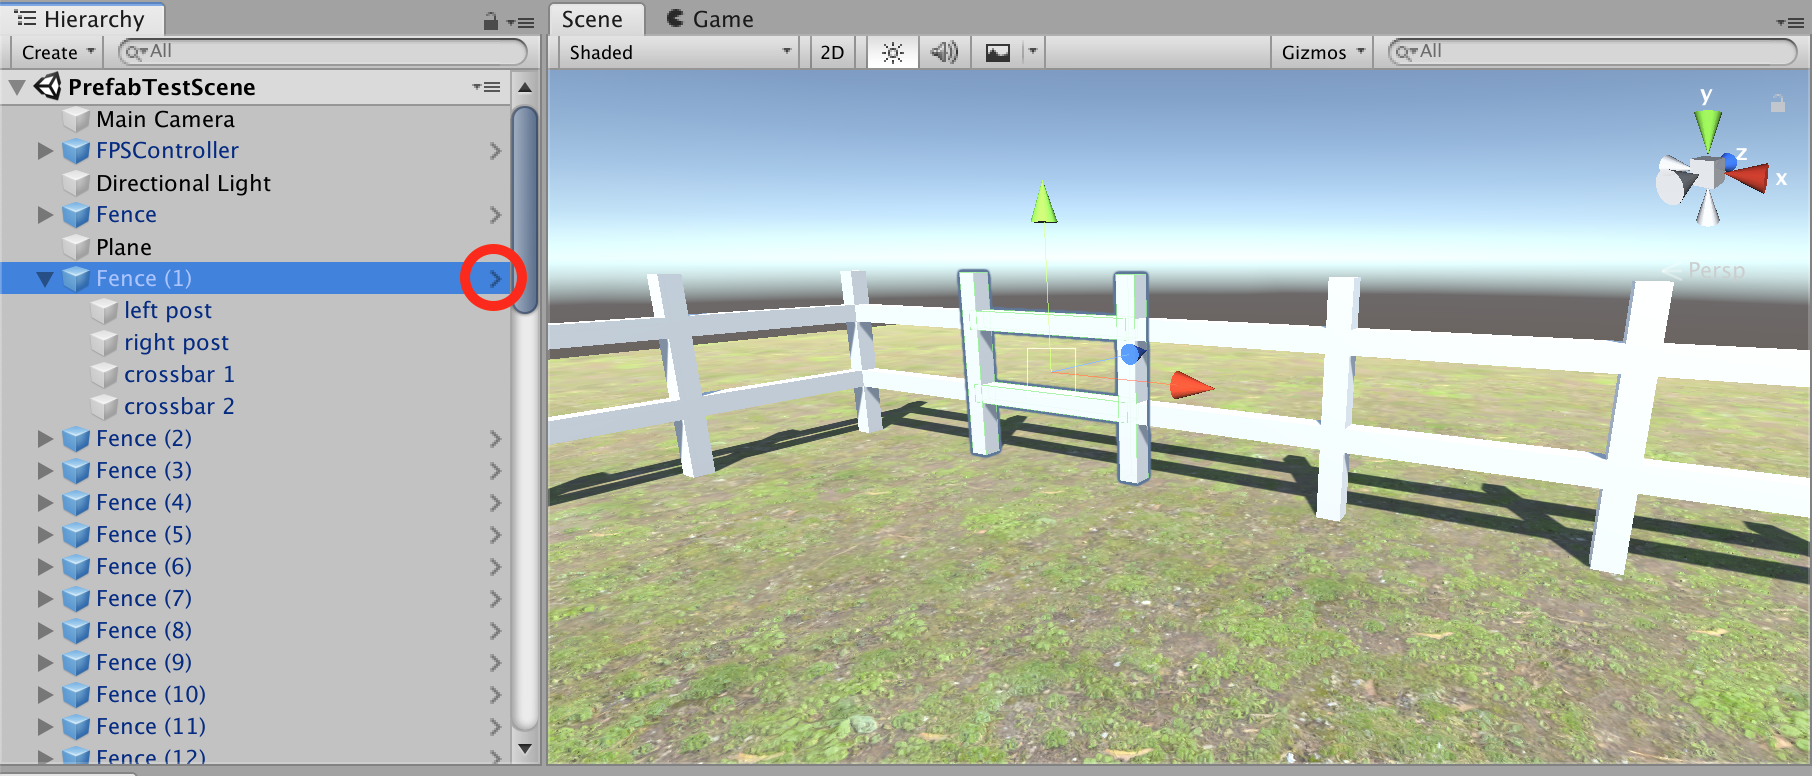
\includegraphics[height=12em]{prefabs-1}
\end{center}

In the above picture we've selected one individual fence link.  Notice how, in the hierarchy view,
the fence GameObjects have a blue box next to them.  This is because each of the fence GameObjects
is \textbf{linked} to a prefab.  The prefab itself is located at 
\directory{ScriptingIntro/PrefabExamples/Fence.asset}.  We can modify the prefab by double clicking
on the prefab file OR clicking on the small arrow next to a fence GameObject at the right side of 
the hierarchy view (circled above).  Unity will then ``jump into'' the prefab so that you can edit
it directly:

\begin{center}
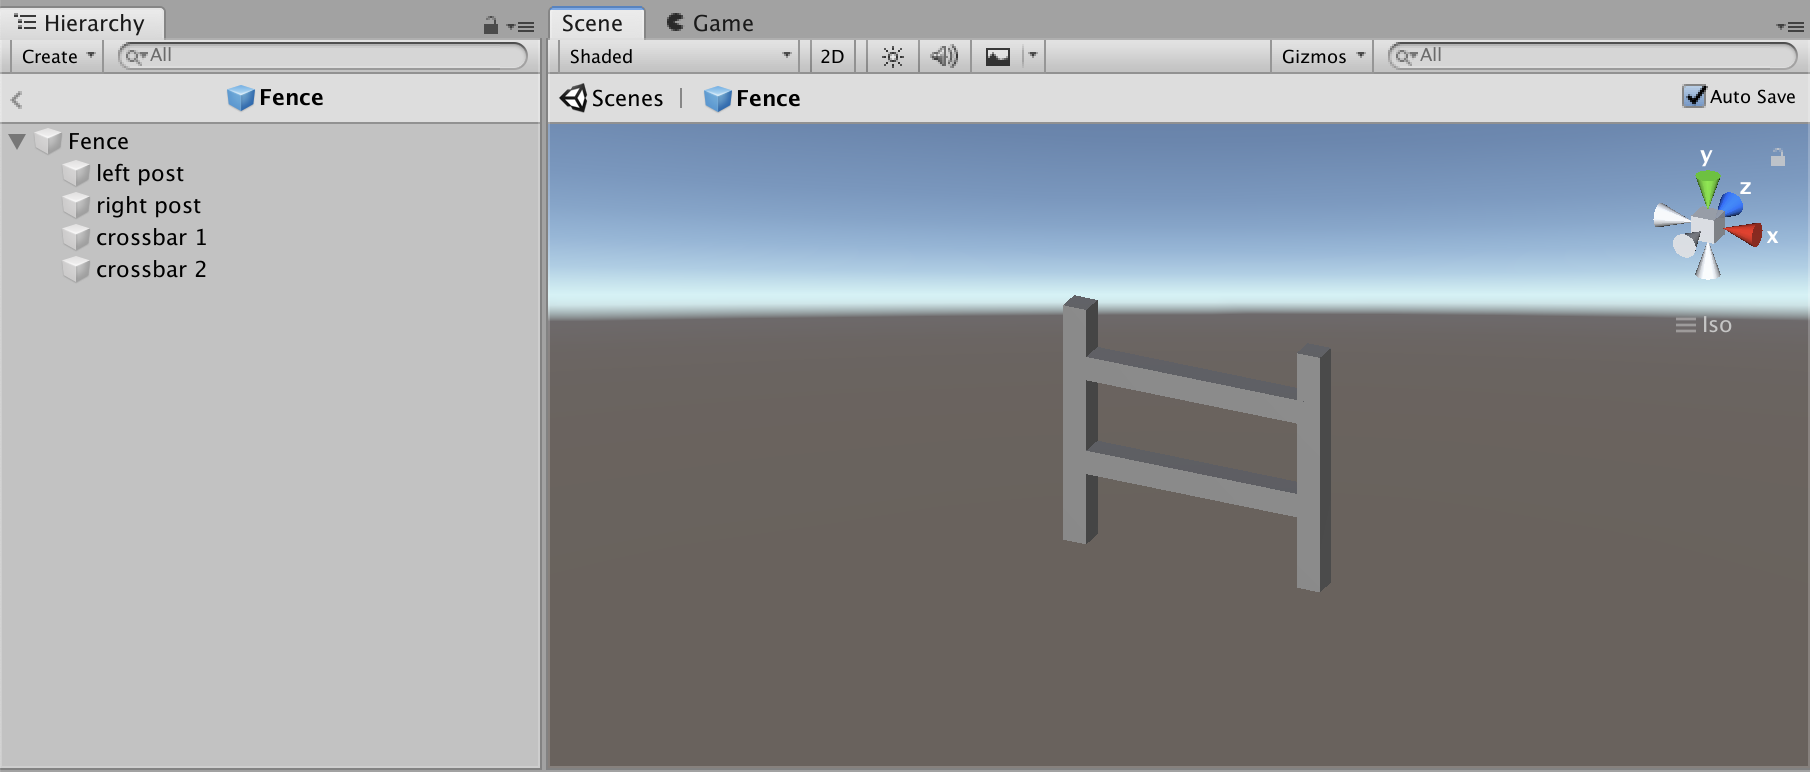
\includegraphics[height=12em]{prefabs-2}
\end{center}

Let's pretend that while working on this game, your team lead complained that the fences look too
boring.  They suggested adding more details to the fences.  If we edit the prefab by adding a crossbar,
then the changes will apply to each instance throughout the scene:

\begin{center}
\raisebox{-.45\height}{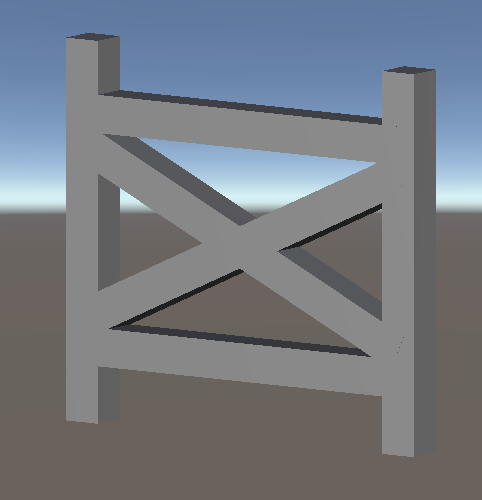
\includegraphics[height=12em]{prefabs-3}} $\rightarrow$
\raisebox{-.45\height}{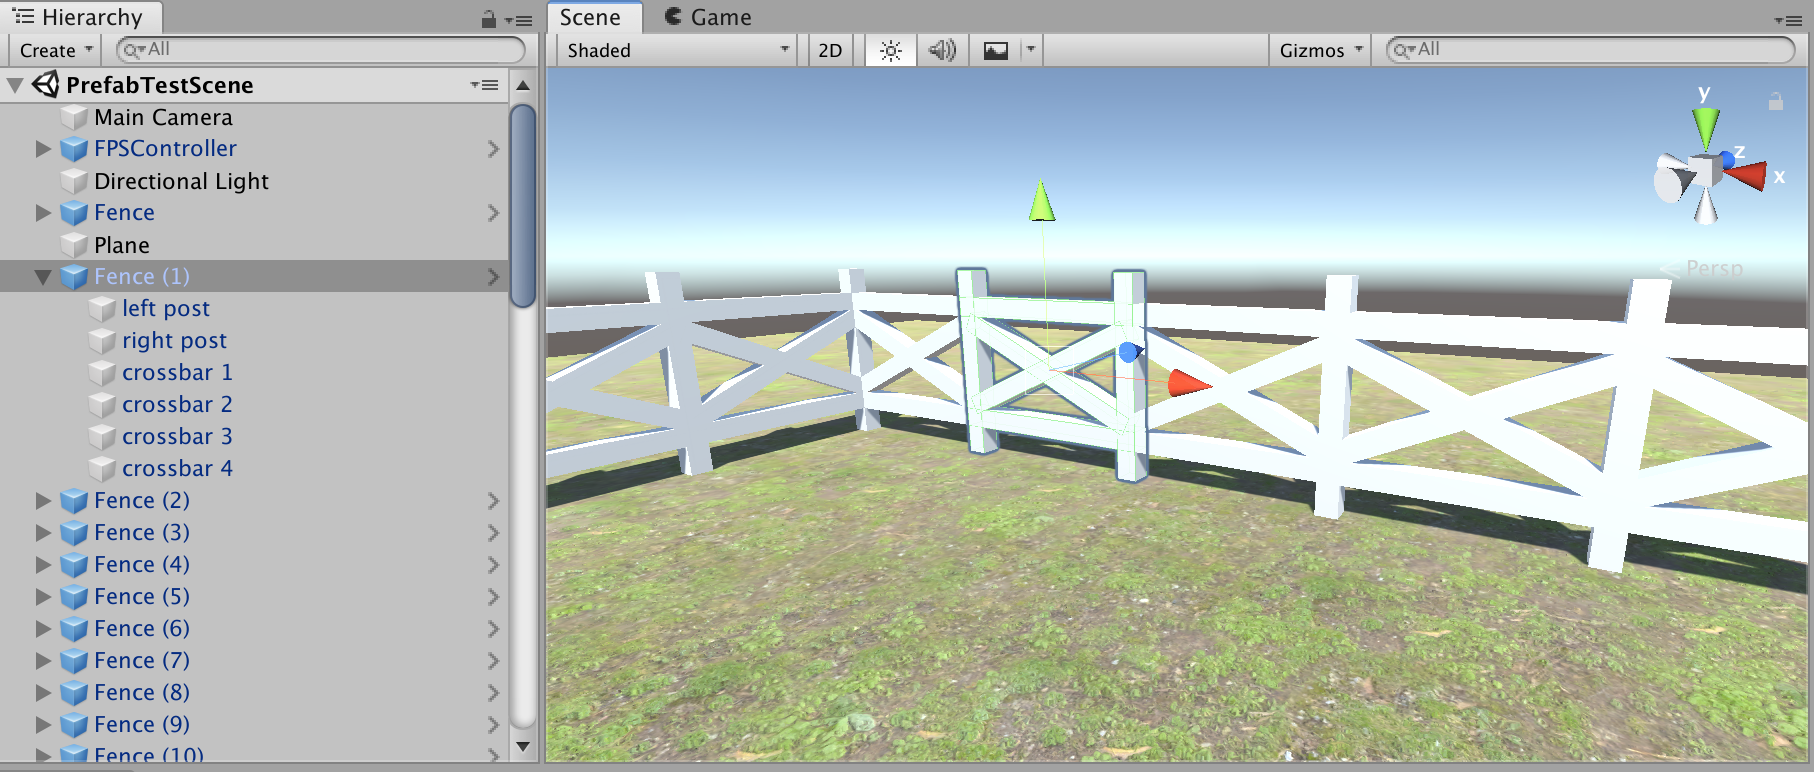
\includegraphics[height=12em]{prefabs-4}} 
\end{center}
\pagebreak
Keep in mind that if we change any of the instances of the fence link in our scene, those changes
will \textbf{override} the prefab version.  For example, if we change the Z-scale of one of our
fence link instances, then change the Z-scale in the prefab to something else, the instance 
will \textit{retain the changes} you made to it:

\begin{center}
\raisebox{-.45\height}{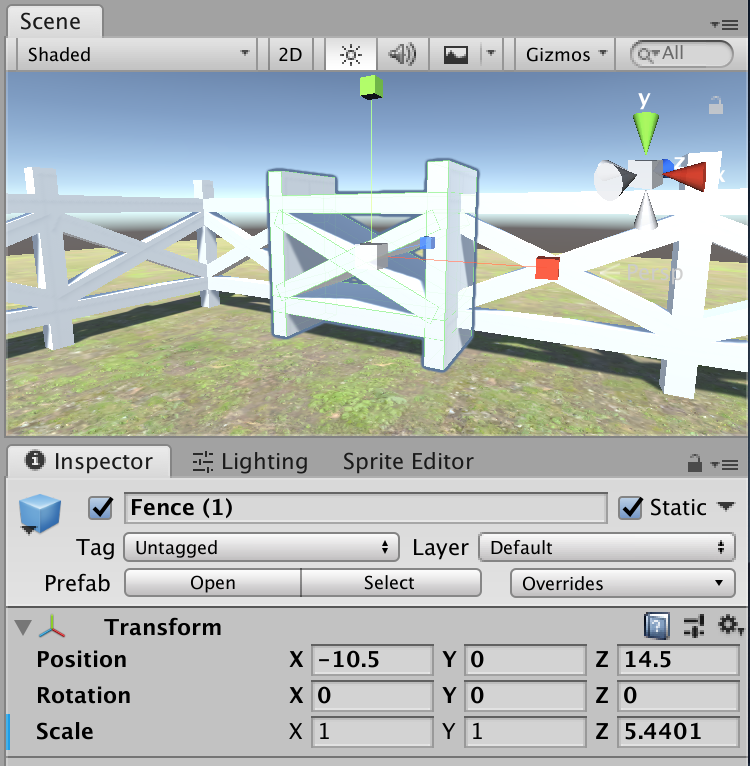
\includegraphics[height=13em]{prefabs-5}} $+$
\raisebox{-.45\height}{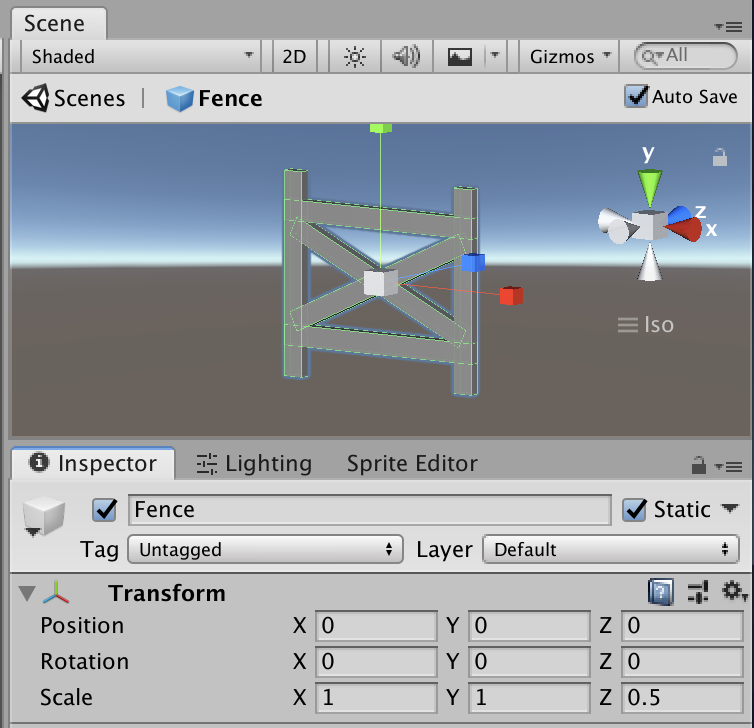
\includegraphics[height=13em]{prefabs-6}} $=$ 
\raisebox{-.45\height}{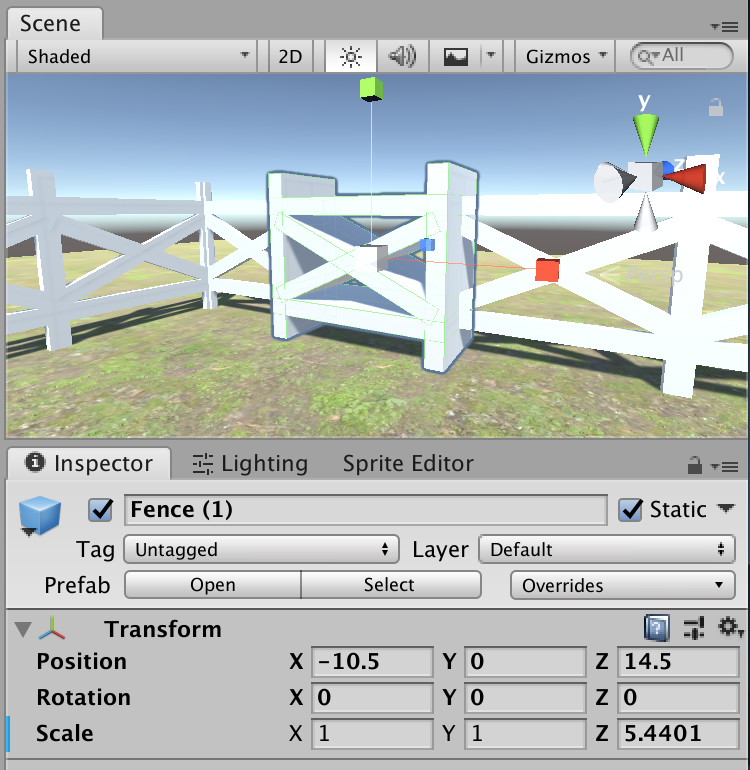
\includegraphics[height=13em]{prefabs-7}} 
\end{center}

Notice how in the above images, the scale field of the instance (see the left and right picture 
above) has a small blue mark to the left of it.  This means that the scale of this object overrides
the prefab.  You can also see which fields are overridden because they are displayed in bold.
You can reset the Z-scale to what is stored in the prefab by right clicking on the field and selecting
``Revert.''  Alternatively you can apply your change to the main prefab by selecting ``Apply to 
Prefab $\dots$''

\begin{center}
\raisebox{-.45\height}{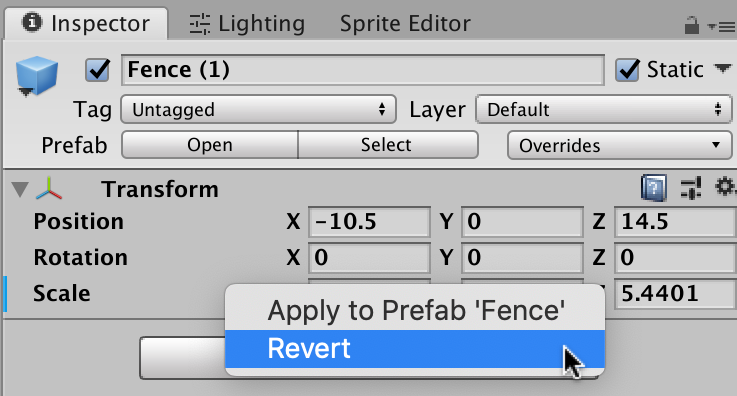
\includegraphics[width=0.35\textwidth]{prefabs-8}} $\rightarrow$
\raisebox{-.45\height}{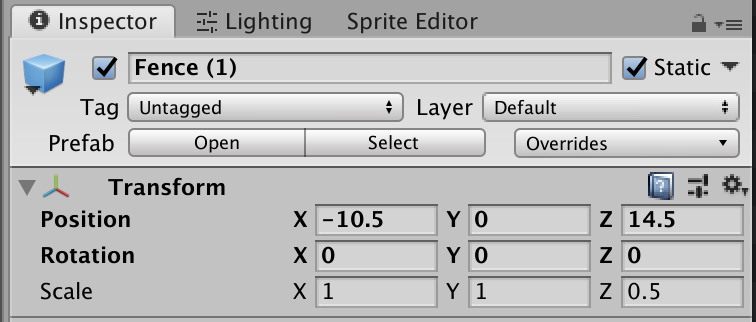
\includegraphics[width=0.35\textwidth]{prefabs-9}}
\end{center}

\subsection{Instantiating Prefabs at Runtime}

You can also use prefabs to \textit{spawn} GameObjects into your scene.  You could use this to spawn
waves of enemies into your levels over time, for example.  There is a command called 
\lstinline|Instantiate<Type>|, available to all \lstinline|MonoBehaviour|s, that creates a copy of
whichever object you pass into it.  The below script spawns a prefab (specified via the field
\lstinline|_PrefabToSpawn|, which is of type \lstinline|GameObject|) into the scene whenever the
player presses a button.  In this case the default is to use \lstinline|Fire1| as the axis, which
is the left mouse button in the default Input Manager configuration (see ``Responding to User 
Input'' above).  In the following example we use \lstinline|Input.GetButtonDown(string)|, 
which is \lstinline|true| only on the first frame that the user presses that button.\pagebreak

\directory{PrefabExamples/SpawnPrefabOnButton.cs}
\StartLineAt{1}
\begin{csharp}
using UnityEngine;

public class SpawnPrefabOnButton : MonoBehaviour
{
    [SerializeField]
    private string _ButtonToPress = "Fire1";
    [SerializeField]
    private GameObject _PrefabToSpawn;
    [SerializeField]
    private Transform _TransformToSpawnAt;

    private void Update()
    {
        if(Input.GetButtonDown(_ButtonToPress))
        {
            var go = Instantiate<GameObject>(_PrefabToSpawn);
            go.transform.position = _TransformToSpawnAt == null ? transform.position : _TransformToSpawnAt.position;
            go.transform.rotation = _TransformToSpawnAt == null ? transform.rotation : _TransformToSpawnAt.rotation;
        }
    }
}
\end{csharp}

You might also want to spawn a prefab every $N$ seconds.  A great way to do this is by using
\textit{Coroutines}.  Coroutines make clever use of C\#'s asynchronous programming features to
\textit{defer execution} of a function to a later frame.  See this Unity manual page for more
information on coroutines:

\begin{center}
\href{https://docs.unity3d.com/Manual/Coroutines.html}{https://docs.unity3d.com/Manual/Coroutines.html}
\end{center}

The next example uses Coroutines to automatically instantiate a prefab every 
\lstinline|_SpawnIntervalSeconds| seconds.  This works because on line 26 we defer execution of
\lstinline|SpawnPrefabCoroutine()| to a later frame.

\directory{PrefabExamples/SpawnPrefabInterval.cs}
\StartLineAt{1}
\begin{csharp}
using System.Collections;
using UnityEngine;

public class SpawnPrefabInterval : MonoBehaviour
{
    [SerializeField]
    private float _SpawnIntervalSeconds = 1.0f;
    [SerializeField]
    private GameObject _PrefabToSpawn;
    [SerializeField]
    private Transform _TransformToSpawnAt;

    private void Start()
    {
        StartCoroutine(SpawnPrefabCoroutine());
    }

    private IEnumerator SpawnPrefabCoroutine()
    {
        while(true)
        {
            var go = Instantiate<GameObject>(_PrefabToSpawn);
            go.transform.position = _TransformToSpawnAt == null ? transform.position : _TransformToSpawnAt.position;
            go.transform.rotation = _TransformToSpawnAt == null ? transform.rotation : _TransformToSpawnAt.rotation;

            yield return new WaitForSeconds(_SpawnIntervalSeconds);
        }
    }
}
\end{csharp}
\pagebreak
\section{Exercise: The Bomb Lab}
\begin{center}
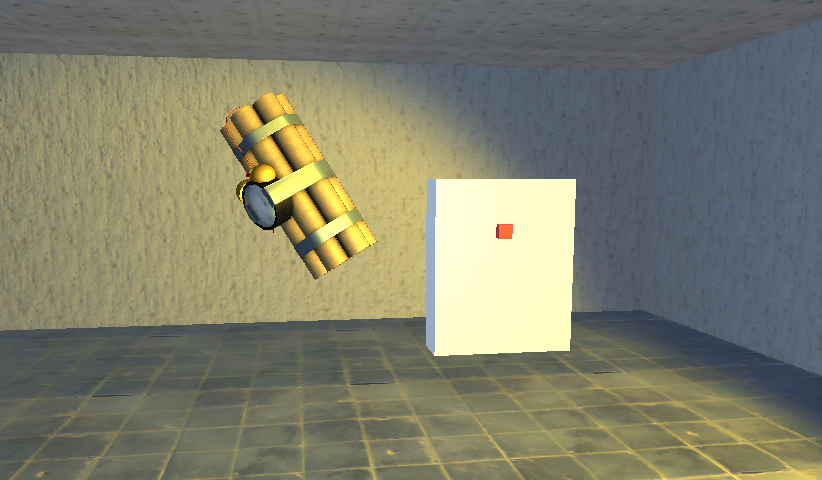
\includegraphics[width=0.5\textwidth]{bomblab-1}
\end{center}
You have been hired by Obedient Cat, a major AAA studio to help out with their next hit game, 
``Previously Mapped 4!''  You sit down to work on your first day when your manager reveals terrible
news: unfortunately the notorious \textit{Dr. Evil} has a vendetta against the company and has 
engaged in cyber terrorism.  Your task today is to defuse a bomb that Dr. Evil has planted in your 
game!

Open the scene located in the base code at \directory{BombLab/BombLab.unity}.  You need to figure 
out how to defuse the bomb.  you'll know the bomb is defused because a message saying 
``DEFUSED!! NICE JOB'' will appear.  As a starting point, I'd recommend taking a look at 
\directory{BombLab/Bomb.cs}.  This file contains the code that makes the bomb work.
\begin{itemize}
    \setlength\itemsep{0.25em}
    \item You may look at the code in \directory{Bomb.cs}, but you \textbf{may not edit it}.
    \item You may move, rotate, or scale any object in the scene.  You may also use ProBuilder to modify the scene.
    \item You \textbf{must} edit the ``Andrew ID'' field of the ``Bomb'' component, which is attached
          to the ``Bomb'' GameObject: \\ 
          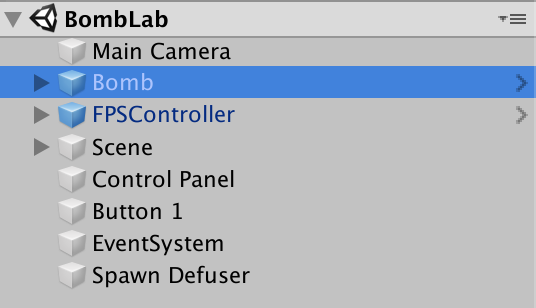
\includegraphics[height=8em]{bomblab-2} 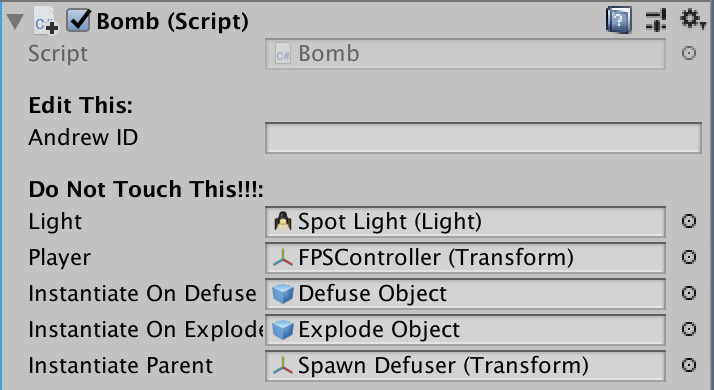
\includegraphics[height=8em]{bomblab-3}
    \item You \textbf{may not} edit any other fields of the ``Bomb'' GameObject (besides the position /
          rotation / scale)
    \item You will probably need to use the UnityEvent exposed by the \textbf{Event On Look And Press}
          script, on the ``Button 1'' GameObject.  This script works similarly to the ``Event On Trigger''
          script discussed above: it triggers the given UnityEvent when the player looks at the button
          and clicks.  Right now, it apparently calls a function called \lstinline|Bomb.Defuse()|.
          Maybe this will defuse the bomb...?  Perhaps, but Dr. Evil is pretty crafty$\dots$\\
          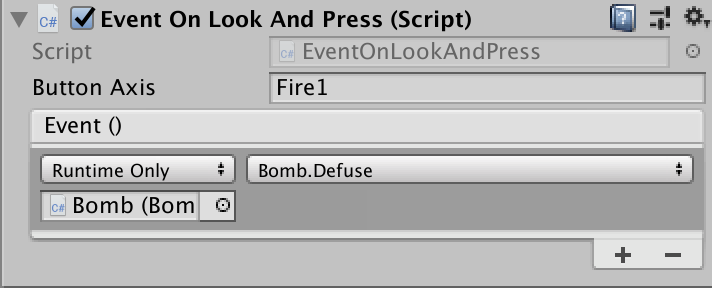
\includegraphics[height=6em]{bomblab-4}
\end{itemize}
\end{document}